\documentclass[a4paper,titlepage]{copin}
\usepackage[portuges,english]{babel}
\usepackage{copin,mestre,epsfig}
\usepackage{times}
\usepackage{multirow}
\usepackage{ucs}
\usepackage[utf8]{inputenc}
\usepackage[T1]{fontenc}
%-----------------------------------------------------------------------------------------------------


\usepackage{fancyheadings}
\usepackage{graphicx}
\usepackage{longtable} %tabelas longas, que ultrapassam uma pagina

\usepackage{listings}
\lstset{numbers=left,
stepnumber=1,
firstnumber=1,
%numberstyle=\tiny,
extendedchars=true,
breaklines=true,
frame=tb,
basicstyle=\footnotesize,
stringstyle=\ttfamily,
showstringspaces=false
}
\renewcommand{\lstlistingname}{C\'odigo Fonte}
\renewcommand{\lstlistlistingname}{Lista de C\'odigos Fonte}

\selectlanguage{portuges}
\sloppy

\begin{document}

%%%%%%%%%%%%%%%%%%%%%%%%%%%%%%%%%%%%%%%%%%%%%%%%%%%%%%%%%%%%%%%%%%%%%%%%%%%%%%%%
\Titulo{Sistemas de Software Artificiais Modulares Realistas}
\Autor{Rodrigo Rocha Gomes e Souza}
\Data{15/03/2010}
\Area{Ciência da Computação}
\Pesquisa{Engenharia de Software}
\Orientadores{Dalton Dario Serey Guerrero  
	 (Orientador) \\
	Jorge César Abrantes de Figueiredo 
	(Orientador)
	}

\newpage
\cleardoublepage

\PaginadeRosto

\newpage
\cleardoublepage

%%%%%%%%%%%%%%%%%%%%%%%%%%%%%%%%%%%%%%%%%%%%%%%%%%%%%%%%%%%%%%%%%%%%%%%%%%%%%%
\begin{resumo} 
% Algoritmos de agrupamento de software agrupam em módulos as entidades do código-fonte de sistemas de software, facilitando a documentação da arquitetura de sistemas. A avaliação empírica desses algoritmos, no entanto, é dificultada pelo fato de existirem poucos sistemas com agrupamentos de referência para serem comparados com os agrupamentos encontrados pelos algoritmos. Neste trabalho é proposta uma abordagem de avaliação usando modelos que produzem grafos que representam sistemas de software organizados em módulos. A abordagem é validada através de um experimento que mostra que os modelos estudados produzem grafos que se assemelham a grafos de dependências estáticas entre entidades de sistemas de software orientados a objetos. Por fim, algoritmos de agrupamento são avaliados através de grafos gerados pelos modelos. Espera-se, com este trabalho, aumentar o conhecimento disponível sobre algoritmos de agrupamento, o que pode contribuir para o seu aperfeiçoamento no futuro.

A análise das dependências entre as entidades do código-fonte de um sistema de software é feita por diversas ferramentas de engenharia reversa com o propósito de revelar informações úteis para a manutenção do software. Existe, no entanto, uma carência de estudos experimentais projetados para avaliar tais ferramentas, em parte devido ao alto custo de se realizar experimentos na área. 

Na área de redes e sistemas distribuídos, o alto custo de experimentação motiva o uso da simulação como meio para avaliar protocolos e algoritmos. Na engenharia reversa, no entanto, simulações são pouco exploradas --- o que se explica parcialmente pela falta de modelos computacionais realistas para dependências entre entidades de código-fonte.

Neste trabalho são apresentados modelos computacionais que geram representações que podem ser interpretadas como dependências entre entidades de código-fonte. Um dos modelos computacionais, chamado BCR+, foi desenvolvido no contexto deste trabalho. Foi desenvolvido também um modelo de classificação que indica, com precisão de 96\%, se uma representação de dependências é realista --- isto é, se ela se assemelha a representações extraídas de sistemas reais. A partir daí foram identificadas configurações de parâmetros para três modelos computacionais (dentre eles, o BCR+) que favorecem a geração de representações realistas.

% Neste trabalho são apresentados três modelos de dependências que podem apoiar a avaliação de ferramentas de engenharia reversa através de simulações controladas. Um dos modelos, chamado BCR+, foi desenvolvido no contexto deste trabalho. Uma avaliação mostrou que, com uma escolha adequada de valores para os parâmetros dos modelos, é possível produzir redes de dependências que se assemelham estruturalmente a redes de dependências extraídas de sistemas de software reais. Ademais, foram derivadas regras que preveem, com 75\% de acurácia, se uma rede gerada com determinada configuração de parâmetros será semelhante a redes extraídas de sistemas de software.

Por fim, é apresentada uma prova de conceito, que demonstra a viabilidade do uso do modelo BCR+ na avaliação de algoritmos usados no contexto de recuperação de arquitetura de software, um ramo da engenharia reversa.

% acurácia de 80%

% <jorge> O resumo carece de números. Acho que já aqui no resumo deve ser mostrado um resumo dos resultados/números. 

% Ao contrário do que ocorre no estudo de redes e sistemas distribuídos, as simulações --- alternativas viáveis aos experimentos quando estes são caros de se realizar --- são pouco exploradas no estudo de ferramentas de engenharia reversa.

% A engenharia reversa, no entanto, carece de modelos realistas para embasar simulações.
\end{resumo}

\newpage
\cleardoublepage

%%%%%%%%%%%%%%%%%%%%%%%%%%%%%%%%%%%%%%%%%%%%%%%%%%%%%%%%%%%%%%%%%%%%%%%%%%%%%%
\begin{summary}
% Software clustering algorithms group source code entities into modules, facilitating software architecture documentation. Empirical evaluation of the algorithms, however, is difficult because there are few software systems with reference clusterings for comparison with the clusterings found by algorithms. In this thesis we propose an approach based on models that generate graphs representing software systems with built-in reference clusterings. The approach is validated through an experiment that shows that the models produce graphs resembling the graph of static dependencies between classes in object oriented software systems. Finally, clustering algorithms are evaluated through model generated graphs. It is expected that this study will increase the available knowledge about clustering algorithms, which can contribute to their improvement in the future.
\end{summary}

\newpage
\cleardoublepage

%%%%%%%%%%%%%%%%%%%%%%%%%%%%%%%%%%%%%%%%%%%%%%%%%%%%%%%%%%%%%%%%%%%%%%%%%%%%%%
\begin{agradecimentos}
Agradecimentos
\end{agradecimentos}

\clearpage

%%%%%%%%%%%%%%%%%%%%%%%%%%%%%%%%%%%%%%%%%%%%%%%%%%%%%%%%%%%%%%%%%%%%%%%%%%%%%%

%% Definicao do cabecalho: secao do lado esquerdo e numero da pagina do lado direito
\pagestyle{fancy}
\addtolength{\headwidth}{\marginparsep}\addtolength{\headwidth}{\marginparwidth}\headwidth = \textwidth
\renewcommand{\chaptermark}[1]{\markboth{#1}{}}
\renewcommand{\sectionmark}[1]{\markright{\thesection\ #1}}\lhead[\fancyplain{}{\bfseries\thepage}]%
	     {\fancyplain{}{\emph{\rightmark}}}\rhead[\fancyplain{}{\bfseries\leftmark}]%
             {\fancyplain{}{\bfseries\thepage}}\cfoot{}

%%%%%%%%%%%%%%%%%%%%%%%%%%%%%%%%%%%%%%%%%%%%%%%%%%%%%%%%%%%%%%%%%%%%%%%%%%%%%%%%
\selectlanguage{portuges}

\Sumario
\ListadeSimbolos
\listoffigures
\listoftables
\lstlistoflistings %lista de codigos fonte - Para inserir a listagem de codigos fonte
\newpage
\cleardoublepage

\Introducao


%%%%%%%%%%%%%%%%%%%%%%%%%%%%%%%%%%%%%%%%%%%%%%%%%%%%%%%%%%%%%%%%%%%%%%%%%%%%%%%%
%
% Hifenizacao - Colocar lista de palavras que nao devem ser separadas e que 
% nao estao no dicionario portugues.
% As palavras do dicionario portugues ja sao separadas corretamente pelo lateX
%
\hyphenation{hardware software}


%%%%%%%%%%%%%%%%%%%%%%%%%%%%%%%%%%%%%%%%%%%%%%%%%%%%%%%%%%%%%%%%%%%%%%%%%%%%%%%%
%% A partir daqui coloque seus capitulos. Sugere-se que eles sejam inseridos com o comando \input
%% Da seguinte maneira:
%%
%% \chapter{Introdu\c{c}\~{a}o}

\section{Se\c{c}\~{a}o 1 do Capítulo 1}
\subsection{Subseção}
\subsubsection{Subsubseção}

A Figura \ref{fig:sistemaProposto}. A Tabela \ref{tab:tabelaTeste}. A Equação (\ref{eq1}). O trabalho de fulano~\cite{ref1}. O Código Fonte \ref{cod1}.

\begin{figure}[htbp]	
\begin{center}
	%	\fbox{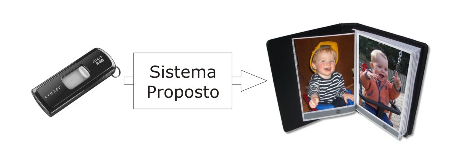
\includegraphics[scale=1]{sistemaProposto.eps}}
	\end{center}
	\caption{Sistema proposto}
	\label{fig:sistemaProposto}
\end{figure}

\begin{table}[htpb]
\begin{center}
\begin{tabular}{|c|c|c|}
\hline
coluna 1 & coluna 2 & coluna 3 \\
\hline
valor 1,1 & valor 1,2 & valor 1,3 \\
valor 2,1 & valor 2,2 & valor 2,3 \\
\hline
\end{tabular}
\end{center}
\caption{Primeira tabela.}
\label{tab:tabelaTeste}
\end{table}

\begin{equation}
E = m \times c^2
\label{eq1}
\end{equation}

\begin{lstlisting}[caption={Loop simples},label=cod1,numbers=none]
for(int x=1; x<10; x++){
  cout << x << "\n";
}
\end{lstlisting}

\section{Se\c{c}\~{a}o 2 do Capítulo 1}  
\subsection{Subseção}
\subsubsection{Subsubseção}

 
%% \input{cap2}
\chapter{Introdu\c{c}\~{a}o}

\section{Se\c{c}\~{a}o 1 do Capítulo 1}
\subsection{Subseção}
\subsubsection{Subsubseção}

A Figura \ref{fig:sistemaProposto}. A Tabela \ref{tab:tabelaTeste}. A Equação (\ref{eq1}). O trabalho de fulano~\cite{ref1}. O Código Fonte \ref{cod1}.

\begin{figure}[htbp]	
\begin{center}
	%	\fbox{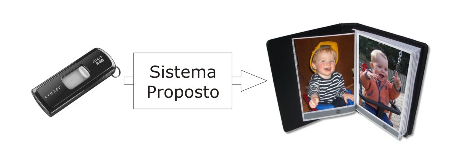
\includegraphics[scale=1]{sistemaProposto.eps}}
	\end{center}
	\caption{Sistema proposto}
	\label{fig:sistemaProposto}
\end{figure}

\begin{table}[htpb]
\begin{center}
\begin{tabular}{|c|c|c|}
\hline
coluna 1 & coluna 2 & coluna 3 \\
\hline
valor 1,1 & valor 1,2 & valor 1,3 \\
valor 2,1 & valor 2,2 & valor 2,3 \\
\hline
\end{tabular}
\end{center}
\caption{Primeira tabela.}
\label{tab:tabelaTeste}
\end{table}

\begin{equation}
E = m \times c^2
\label{eq1}
\end{equation}

\begin{lstlisting}[caption={Loop simples},label=cod1,numbers=none]
for(int x=1; x<10; x++){
  cout << x << "\n";
}
\end{lstlisting}

\section{Se\c{c}\~{a}o 2 do Capítulo 1}  
\subsection{Subseção}
\subsubsection{Subsubseção}

 
% (5-10) páginas
%
%   Objetivos geral e específicos
%   Resultados esperados
%   Limitações do trabalho
%   Métodos
%   Justificativa
%   Descrição dos demais capítulos

% In practice, there are two kinds of software dependencies:	Static, or "compile-time," dependencies and dynamic, or "run-time," dependencies.
% Static dependencies capture the notion that one software module is necessary in order to compile another. In other words, A depends on B just in case the source code of A makes an explicit reference to B. In such a case, in order to compile A to an executable form, it is necessary to have access to B.
% Run-time dependencies, in contrast, are based on actual calling patterns of the software during operation, and vary according its use and deployment. They cannot, in general, be inferred from any a priori examination of the software code. For this reason, this investigation focuses on analyzing static software dependencies.

\chapter{Introdução}

\begin{section}{Motivação}

		Para um sistema de software ser bem sucedido não basta ele ser rápido, funcional e isento de defeitos. Esses atributos dizem respeito à qualidade, da forma como é enxergada pelos seus usuários, de uma versão do sistema. Para atender a demandas emergentes de seus usuários e incorporar novidades tecnológicas, no entanto, um sistema de software deve apresentar certos atributos de qualidade interna, visíveis apenas para os seus desenvolvedores. Ele precisa ser fácil de compreender, fácil de modificar e fácil de testar \cite{Parnas1994}.

		Um bom indicador da qualidade interna de um sistema de software é a estrutura de dependências entre as entidades que compõem o seu código-fonte. É natural que existam interações entre diversas entidades em um sistema, mas dependências indesejadas adicionam complexidade ao sistema, tornando mais difíceis as tarefas de compreender ou testar isoladamente as diversas partes do sistema.

		Analisar uma a uma as dependências de um sistema de software com a finalidade de extrair informações que apoiem a sua modificação é, no entanto, é uma tarefa árdua \cite{Tonella2007}. Para automatizar essa tarefa, diversas ferramentas de engenharia reversa têm sido propostas. As ferramentas buscam identificar, entre outros, partes do sistema afetadas por uma mudança \cite{Arnold1993}, código duplicado \cite{Roy2007} e módulos arquiteturais \cite{Maqbool2007}.

	As tarefas que as ferramentas de engenharia buscam automatizar, entretanto, envolvem alguma subjetividade, e por isso as ferramentas precisam ser avaliadas empiricamente. A frequência com que as avaliações empíricas são realizadas, contudo, está aquém do que se espera de uma área de pesquisa madura \cite{Tonella2007}. Um estudo realizado sobre artigos sobre engenharia reversa publicados de 2002 a 2005 revelou que 25\% dos artigos não apresentam qualquer forma de avaliação empírica e, dentre os demais artigos, apenas 30\% recorrem a experimentos e estudos observacionais --- os outros 70\% se limitam a estudos de caso e relatos de experiência.

		A escassez de experimentos controlados em engenharia reversa pode ser explicada, em parte, pelo alto custo envolvido na realização de experimentos de qualidade. Em muitos casos, os experimentos envolvem um planejamento cuidadoso e dependem da disponibilidade de desenvolvedores experientes.

		Uma abordagem empregada quando os experimentos controlados são caros é a simulação baseada em modelos computacionais e estatísticos. Na área de redes e sistemas distribuídos, por exemplo, é frequente o uso de ambientes de simulação de redes, que modelam o funcionamento de uma rede de computadores, incluindo, às vezes, modelos de falhas de hardware e até modelos de comportamento de usuários \cite{White2002}. A simulação oferece um meio para se realizar experimentos controlados a um custo baixo. (Naturalmente, há o risco de os modelos usados na simulação não corresponderem à realidade nos aspectos relevantes para o experimento).

		Na engenharia de software, a abordagem de modelagem e simulação já foi usada no estudo de processos de desenvolvimento XXX, mas em geral é uma abordagem pouco explorada. Se protocolos de rede podem ser avaliados em experimentos simulados com modelos de redes de computadores, por que não avaliar ferramentas de engenharia reversa com base em dependências que foram construídas a partir da simulação controlada de um modelo de dependências?
		
\end{section}

\begin{section}{Objetivos}
	O objetivo desta pesquisa é descobrir e avaliar modelos de dependências entre entidades do código-fonte de sistemas de software com a finalidade de apoiar o uso de simulações na avaliação de técnicas de engenharia reversa que se baseiam na análise de dependências.
	
	Para atingir o objetivo de pesquisa é necessário cumprir os seguintes objetivos específicos:
	
	\begin{enumerate}
		\item descobrir modelos que podem ser interpretados como modelos de dependências entre entidades de código-fonte;
		\item avaliar os modelos de acordo com a similaridade entre a estrutura das dependências produzidas pelos modelos e a estrutura das dependências que são extraídas de sistemas de software reais;
		\item realizar uma prova de conceito para demonstrar a viabilidade da abordagem de simulação para a avaliação de técnicas e ferramentas que se baseiam na análise de dependências.
	\end{enumerate}
	
	A fim de melhor representar a forma como sistemas de software são idealizados e construídos, optamos por considerar modelos em que as entidades de código-fonte estão organizadas em módulos. % ficou muito seco? desculpa esfarrapada?
	
\end{section}

\begin{section}{Métodos e Resultados}
	
	A teoria das redes complexas estuda métodos para analisar redes (ou grafos) encontradas nos mais diversos domínios, como redes sociais, redes de computadores e redes metabólicas. A aplicação de tais métodos levou à descoberta de propriedades comuns a um grande número de redes, bem como modelos de redes que incorporam essas propriedades.
	
	Dado que as dependências em um sistema de software formam uma rede, é possível aplicar nesta pesquisa alguns dos métodos, modelos e descobertas da teoria das redes complexas, os quais são apresentados no Capítulo \ref{cap:redes}.
	
	Foram encontrados na literatura dois modelos de redes organizadas em módulos, denominados CGW e LFR, os quais podem ser interpretados como modelos de dependências entre entidades de software. Esses modelos são apresentados no Capítulo \ref{cap:redes}. Um terceiro modelo, o BCR+, foi desenvolvido no contexto desta pesquisa. O modelo BCR+ é descrito em detalhes no Capítulo \ref{cap:bcr}.
	
	A avaliação dos modelos, descrita no Capítulo \ref{cap:avaliacao}, teve como base a simulação dos três modelos. As redes produzidas pelos modelos foram comparadas com redes de dependências extraídas de sistemas de software escritos em uma linguagem de programação orientada a objetos. Os resultados indicam que, com uma escolha adequada de parâmetros, os três modelos produzem redes que se assemelham a redes de dependências entre entidades de software (ao menos no caso de linguagens de programação orientadas a objetos).
	
	Para a prova de conceito foi escolhido o problema de recuperação de arquitetura de software. Algoritmos de agrupamento usados na atividade de recuperação de arquitetura foram aplicados a redes de dependências geradas pelo modelo BCR+ e os resultados foram analisados. No Capítulo \ref{cap:estudo} é feita uma introdução ao problema de recuperação de arquitetura e, a seguir, são apresentados os métodos e resultados da prova de conceito.
	
	No Capítulo \ref{cap:trabrel} este trabalho é comparado a trabalhos relacionados. No Capítulo \ref{cap:conclusao} são apresentadas as conclusões, contribuições e limitações deste trabalho.
	
	% Como resultado, foram encontrados dois modelos de redes apropriados para representar dependências entre entidades, e um modelo que foi criado a partir da adaptação de um modelo existente. O novo modelo é apresentado em detalhes no Capítulo ....
	% 
	% A avaliação dos modelos foi realizada através da simulação dos modelos e posterior uso de métodos asd.sd..asd.... Linguagens OO apenas. A avaliação e os resultados são apresentados no Capítulo ....
	% 
	% Para a prova de conceito foi escolhido o problema de recuperação de arquitetura. A prova de conceito .. no Capítulo ....
	
\end{section}

% (15-25)
%
% DESIGN DE SOFTWARE
% DEFINIR REDE DE SOFTWARE
% CLUSTERING
% AVALIAÇÃO DE CLUSTERING
% 
%     * redes complexas
%     * designs de software como redes complexas
%     * conceito de tríadas como base para caracterização de redes complexas
%     * clustering
%     * avaliação de algoritmos de clustering

\chapter{Agrupamento de Software} \label{cap:agrupamento}

% TODO: Onde falar sobre extração do design?

\begin{section}{Recuperação de Arquitetura de Software}

A arquitetura de um sistema de software é formada pelas decisões mais significativas sobre o desenvolvimento do sistema [Booch, 2006]. Essas decisões devem ser tomadas preferencialmente nos estágios iniciais do processo de desenvolvimento, pois elas afetam um grande número de decisões ao longo do ciclo de vida do software.

É comum documentar uma arquitetura como um conjunto de visões, na qual cada visão descreve decisões que dizem respeito a um subconjunto dos requisitos do sistema \cite{Clements2002}. A visão modular é a mais importante no gerenciamento da evolução de software \cite{Parnas1972}. Ela representa a organização de um sistema em módulos com responsabilidades bem definidas e descreve interações entre os módulos. A visão modular facilita a análise de atributos como facilidade de modificação e possibilidade de reuso de partes do sistema.

Muitos sistemas, no entanto, não possuem uma arquitetura bem documentada. Durante o desenvolvimento de um sistema, a documentação de sua arquitetura pode tornar-se desatualizada, resultando em uma deterioração da estrutura do sistema \cite{Eick2001,Parnas1994}. O problema se agrava quando os desenvolvedores originais abandonam o projeto, levando com eles um conhecimento tácito sobre a arquitetura do sistema.

O termo recuperação de arquitetura (ou reconstrução de arquitetura) se refere a métodos que extraem aspectos da arquitetura de um sistema a partir de artefatos criados durante seu desenvolvimento, como o código-fonte \cite{Pollet2007}. Tais métodos têm sido usados como auxílio em tarefas como a documentação da arquitetura e a compreensão de sistemas legados \cite{Wu2005}.

Uma abordagem bastante pesquisada para auxiliar a compreensão e a documentação da visão modular da arquitetura de sistemas é chamada agrupamento de software \cite{Mancoridis1998,Andritsos2005,Maqbool2007}. Algoritmos de agrupamento de software agrupam o conjunto de entidades do código-fonte de um sistema (por exemplo, classes em um sistema orientado a objetos) em subconjuntos denominados módulos. O agrupamento é feito de forma que, sob algum critério, as entidades agrupadas em um mesmo módulo possuem grande similaridade entre si e pequena similaridade com entidades que estão em outros módulos. Vale ressaltar que o termo agrupamento designa tanto a atividade de agrupamento como o resultado dessa atividade, que é a organização das entidades analisadas em módulos.

Naturalmente, o problema de agrupar entidades segundo algum critério de similaridade não é exclusivo do domínio de software. O problema tem sido objeto da mineração de dados, da inteligência artificial, do estudo de redes sociais etc. Assim como em outros domínios, o problema de agrupamento de software não é bem definido no domínio de recuperação de arquitetura. A definição de qual é o melhor agrupamento é subjetiva. Ainda assim, o agrupamento dos dados pode evidenciar relacionamentos existentes entre entidades e servir como ponto de partida de atividades como, por exemplo, a atribuição de arquivos de código-fonte a programadores.

% Falar sobre escolha das entidades e da descrição das entidades (citar Anquetil antigo, que usa nome de arquivo, e Anquetil novo, que compara resultados de diversas descrições, e Kuhn2005). AQUI? Onde?

\end{section}

\begin{section}{Algoritmos de Agrupamento de Software}

Para realizar o agrupamento automático de um conjunto de entidades, as seguintes questões devem ser consideradas:

\begin{itemize}
	\item a identificação das entidades;
	\item a descrição das entidades;
	\item o algoritmo de agrupamento;
\end{itemize}

No domínio do agrupamento de software, exemplos de entidades incluem, entre outros, arquivos fonte \cite{Mancoridis1998}, funções e variáveis em sistema procedimentais \cite{Anquetil1999} e classes em um sistema orientado a objetos \cite{Trifu2001} etc.

A descrição das entidades determina as características a se considerar para determinar se duas entidades são mais ou menos similares. Por exemplo, se o objetivo é agrupar funções em um programa procedimental, as seguintes descrições, entre outras, podem ser adotadas para cada entidade:

\begin{itemize}
	\item conjunto das palavras usadas nos comentários que descrevem a função;
	\item conjunto dos programadores que trabalharam na função;
	\item conjunto das funções chamadas pela função;
	\item conjunto das variáveis manipuladas na função.
\end{itemize}

As duas últimas descrições são chamadas de descrições formais, pois elas têm impacto sobre o comportamento do programa, e são as descrições mais estudadas \cite{Anquetil1999}. Em muitos casos, a descrição formal de um sistema é representada como grafo. As duas primeiras descrições são ditas não-formais. 

% XXX
% Após a identificação das entidades a serem agrupadas, portanto, o processo de agrupamento é realizado em duas etapas: a extração das descrições das entidades e o agrupamento propriamente dito. A Figura XXX ilustra o processo, considerando uma descrição sob a forma de grafo.
% 
% \begin{figure}[htbp]
% 	\centering
% 		\includegraphics[scale=1]{file}
% 	\caption{caption}
% 	\label{fig:label}
% \end{figure}

A seguir são descritos brevemente alguns algoritmos que têm sido pesquisados no contexto de agrupamento de software, com foco em descrições formais de software. Para esta pesquisa foram escolhidos algoritmos estudados por diferentes grupos de pesquisa e com implementação disponível publicamente.

\begin{subsection}{Algoritmos Hierárquicos Aglomerativos}

Algoritmos hierárquicos aglomerativos têm sido aplicados a diversos problemas, incluindo o agrupamento de software \cite{Anquetil1999,Maqbool2007}. Essa família de algoritmos funciona com qualquer descrição de entidade, desde que seja fornecida uma métrica de similaridade entre pares de entidades. A similaridade entre duas entidades é medida em uma escala contínua de 0 a 1. O algoritmo é simples: inicia-se com um módulo para cada entidade e então mesclam-se sucessivamente os dois módulos mais similares até restar apenas um módulo com todas as entidades.

No contexto de recuperação de arquitetura de software, é comum descrever as entidades de código-fonte como um grafo de dependências entre entidades e usar a métrica de Jaccard para medir a similaridade entre duas entidades \cite{Anquetil1999}. Sejam X e Y duas entidades, e seja d(A) o conjunto de entidades ligadas à entidade A no grafo de dependências. A similaridade entre X e Y é dada pela expressão a seguir:

$$
\mathrm{sim}(X, Y) ~=~ \frac{|\mathrm{d}(X) \cap \mathrm{d}(Y)|}{|\mathrm{d}(X) \cup \mathrm{d}(Y)|}
$$

O que diferencia os algoritmos hierárquicos aglomerativos entre si é o critério usado para medir a similaridade entre dois módulos. Os dois critérios mais estudados no contexto de agrupamento são chamados de ligação simples (SL, do inglês \emph{single linkage}) e ligação completa (CL, do inglês \emph{complete linkage}). Na ligação simples, a similaridade entre dois módulos é computada como a maior similaridade entre pares de entidades tiradas uma de cada módulo. Na ligação completa é considerada a menor similaridade.

Naturalmente, um agrupamento que consiste de apenas um módulo com todas as entidades analisadas é de pouco valor. Por essa razão deve existir um critério de parada que interrompa o algoritmo de todos os módulos serem mesclados em um grande módulo. No contexto de agrupamento de software, o critério mais comumente usado é a altura de corte, $h$, que varia entre 0 e 1. Sob esse critério, o algoritmo interrompe sua execução quando a maior similaridade entre dois módulos é igual a $1 - h$. Assim, quanto maior a altura de corte $h$, menor o número de módulos do agrupamento resultante.
	
\end{subsection}

%%%%%%%%%

\begin{subsection}{Bunch}

Com a finalidade de auxiliar a compreensão de programas, o algoritmo Bunch \cite{Mancoridis1998} agrupa o conjunto de entidades de um programa de acordo com os relacionamentos existentes entre elas, representados como um grafo orientado. O agrupamento é tratado como um problema de otimização no qual o objetivo é maximizar uma função denominada qualidade de modularização (QM), que recompensa agrupamentos com muitas arestas internas (que ligam entidades de um mesmo módulo) e poucas arestas externas (que ligam entidades de módulos distintos).

% TODO: fórmula da QM

Encontrar um agrupamento que possui QM ótima é um problema intratável; por isso a ferramenta usa heurísticas como algoritmos genéticos e \emph{hill-climbing} para obter resultados quase ótimos.

\end{subsection}

%%%%%%%%%%

\begin{subsection}{ACDC}

O algoritmo ACDC \cite{Tzerpos2000} foi projetado com o intuito de encontrar agrupamentos que facilitam a compreensão de programas. Assim como o Bunch, ele opera sobre grafos orientados. Sua principal característica é a identificação de conjuntos dominantes de vértices no grafo. Um conjunto dominante é um conjunto de vértices, $v_0, v_1, \ldots{}, v_n$, onde $v_0$ é o vértice dominante, que satisfaz a duas condições: (i) existe um caminho entre $v_0$ e qualquer $v_i$; (ii) qualquer caminho de um vértice que não pertence ao conjunto até um vértice do conjunto, $v_i$, passa por $v_0$. O algoritmo ACDC identifica os conjuntos dominantes, em ordem crescente de número de vértices, e considera-os módulos do agrupamento. 

% subgraph dominator
% evita módulos muito grandes.
	
\end{subsection}

\end{section}

\begin{section}{Avaliação de Algoritmos de Agrupamento}

Como já foi mencionado, não existe um critério objetivo para determinar qual é o melhor agrupamento das entidades de um sistema de software. Ainda assim, alguma forma de avaliação de algoritmos de agrupamento é necessária para comparar os diferentes algoritmos. Uma das formas de avaliar os agrupamentos produzidos por algoritmos comparando-os com agrupamentos de referência, produzidos por especialistas, do conjunto de sistemas nos quais os algoritmos foram executados \cite{Koschke2000}.

A Figura \ref{fig:mojo} ilustra dois agrupamentos de um mesmo sistema de software hipotético, representado como um grafo orientado que descreve dependências estáticas entre classes do sistema. É fácil perceber que os agrupamentos não são idênticos: um deles possui quatro módulos, enquanto o outro possui três. Ainda assim, os agrupamentos são bastante semelhantes. O módulo $M_4$ corresponde exatamente ao módulo $M_C$; O módulo $M_3$ é quase igual ao módulo $M_B$; e os módulos $M_1$ e $M_2$, unidos, são parecidos com o módulo $M_A$.

\begin{figure}[htbp]
	\centering
		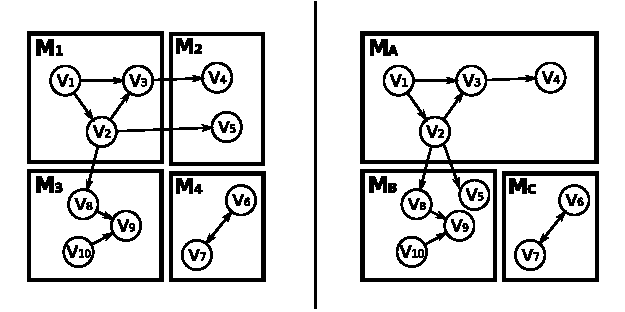
\includegraphics[scale=1]{figuras/redes-dupla}
	\caption{Dois agrupamentos de um mesmo sistema de software hipotético, descrito como um grafo que representa dependências entre classes.}
	\label{fig:mojo}
\end{figure}

% É fácil verificar se dois agrupamentos de um mesmo conjunto de entidades são idênticos ou não. Para comparar diferentes agrupamentos produzidos por algoritmos, no entanto, é preciso definir uma métrica de similaridade entre agrupamentos que seja capaz de determinar qual agrupamento de uma coleção de agrupamentos é mais similar a um agrupamento de referência.

No domínio de agrupamento de software, a métrica MoJo \cite{Tzerpos1999} tem sido bastante utilizada para medir a similaridade entre dois agrupamentos. A ideia por trás da métrica é que um agrupamento dado é muito similar a um agrupamento de referência se é possível transformar o primeiro agrupamento no segundo usando poucas operações do tipo mover e mesclar. A operação mover consiste de mover uma entidade de um módulo para outro módulo distinto. A operação mesclar consiste de mesclar dois módulos. O MoJo entre  dois agrupamentos é igual ao número de operações de mover e mesclar que são necessárias para transformar o primeiro agrupamento no segundo. Quanto menor o MoJo, maior a similaridade entre dois agrupamentos; agrupamentos idênticos têm MoJo igual a zero.

A métrica MoJo não é simétrica. Para chegar a essa conclusão, basta observar que há uma operação de mesclar módulos, mas não uma operação de dividir um módulo em dois. No contexto de avaliação de algoritmos de agrupamento de software, é considerado o número de operações necessárias para transformar o agrupamento encontrado por um algoritmo no agrupamento de referência.

Na Figura \ref{fig:mojo}, considerando que o agrupamento de referência é o segundo (o da direita), o MoJo entre os dois agrupamentos vale 2. Para transformar o primeiro agrupamento no segundo são necessárias, portanto, duas operações: mesclar os módulos $M_1$ e $M_2$, e mover o vértice $v_5$ para o módulo $M_3$. Após a realização dessas operações, os agrupamentos se tornam idênticos, considerando as correspondências $(M_1 \cup M_2) = M_A$, $M_3 = M_B$ e $M_4 = M_C$.

Observando que o valor MoJo entre dois agrupamentos com o mesmo número de entidades varia entre 0 e o número de entidades em cada agrupamento, $n$, é possível definir uma métrica, chama MoJoSim, que mapeia o valor MoJo em uma escala de 0 a 1 \cite{Bittencourt2009}. O valor 0 representa a menor similaridade e o valor 1, a maior similaridade. O valor de MoJoSim entre dois agrupamentos é definido de acordo com a seguinte equação:

$$
\mathrm{MoJoSim}(X, Y) ~=~ 1 - \frac{\mathrm{MoJo}(X, Y)}{n}
$$

% Anquetil avaliou 

Wu, Hassan e Holt \cite{Wu2005} avaliaram os algoritmos Bunch, ACDC e algoritmos aglomerativos comparando, através da métrica MoJo, os agrupamentos encontrados pelos algoritmos com agrupamentos de referência de 5 sistemas de software em C e C++, representados como um grafo dos arquivos fonte e dependências estáticas entre os arquivos. Os agrupamentos de referência foram obtidos automaticamente a partir de uma análise da estrutura de diretórios dos sistemas. Cada diretório contendo pelo menos 5 arquivos fonte foi considerado um módulo do sistema. Bittencourt e Guerrero \cite{Bittencourt2009} realizaram um experimento semelhante, porém avaliando algoritmos de agrupamento estudados em outros domínios aplicados sobre um conjunto de 4 sistemas em Java.

\end{section}


% \begin{section}{Agrupamento}
% 
% A atividade de agrupamento consiste de agrupar um conjunto de entidades em subconjuntos, denominados módulos, de forma que, sob algum critério, as entidades agrupadas em um mesmo módulo possuem grande similaridade entre si e pequena similaridade com entidades que estão em outros módulos. Em muitas aplicações, a noção de módulo não é bem definida. Ainda assim, o agrupamento dos dados pode evidenciar relacionamentos existentes entre entidades e servir como ponto de partida de atividades como, por exemplo, a atribuição de arquivos de código-fonte a programadores.
% 
% O termo agrupamento designa tanto a atividade de agrupamento como o resultado dessa atividade, que é a organização das entidades analisadas em módulos. Existem diversos tipos de agrupamento:
% 
% \begin{itemize}
% 	\item hierárquico vs. partitivo: no agrupamento hierárquico, os módulos são sucessivamente agrupados em módulos de módulos. No agrupamento partitivo, apenas as entidades estão agrupadas em módulos. Uma organização hierárquica pode ser transformada em plana se a árvore da hierarquia for cortada em algum nível.
% 
% 	\item completo vs. parcial: na organização completa, todas as entidades pertencem a algum módulo; na organização parcial podem existir entidades sem módulos.
% 
% 	\item módulos sobrepostos vs. mutuamente exclusivos: na organização com módulos sobrepostos, podem existir entidades que pertencem a mais de um módulo; na organização de módulos mutuamente exclusivos, cada entidade pertence a no máximo um módulo.
% \end{itemize}
% 
% %%%%%%%% SIMILARIDADE
% 
% Para realizar o agrupamento de um conjunto de entidades de maneira sistemática, as seguintes questões devem ser consideradas:
% 
% \begin{itemize}
% 	\item identificação das entidades;
% 	\item a descrição das entidades;
% 	\item o algoritmo de agrupamento;
% \end{itemize}
% 
% A descrição das entidades determina as características a se considerar para determinar se duas entidades são mais ou menos similares. Por exemplo, se o objetivo é agrupar funções em um programa procedimental, as entidades são funções e as seguintes descrições, entre outras, podem ser adotadas para cada entidade:
% 
% \begin{itemize}
% 	\item conjunto das palavras usadas nos comentários que descrevem a função;
% 	\item conjunto dos programadores que trabalharam na função;
% 	\item conjunto das funções chamadas pela função;
% 	\item conjunto das variáveis manipuladas na função.
% \end{itemize}
% 
% As duas últimas descrições são chamadas de descrições formais, pois elas têm impacto sobre o comportamento do programa \cite{Anquetil1999}. As duas primeiras são descrições não-formais. 
% 
% Algoritmos de agrupamento são estudados em áreas diversas como a mineração de dados, a física estatística, a inteligência artificial e a engenharia de software. Alguns algoritmos são genéricos e dependem apenas de um conjunto de entidades e de uma função que define a similaridade entre entidades. Outros algoritmos são específicos para grafos.
% 
% \end{section}
% 
% \begin{section}{XXX}
% 
% Muitas abordagens de recuperação de arquitetura são baseadas na análise de código-fonte \cite{Pollet2007}. Uma parte destas abordagens usa algoritmos de clustering para determinar um agrupamento das entidades do código-fonte. Nesses trabalhos, as entidades podem ser funções e variáveis em sistema procedimentais CITE, tipos abstratos de dados CITE, arquivos-fonte CITE, classes em um sistema orientado a objetos CITE etc. Em outra dimensão, vários descrições são usadas para as entidades: nomes de identificadores CITE, co-mudança em sistemas de controle de versão CITE, co-uso em tempo de execução CITE, dependências estáticas no código-fonte etc.
% 
% Neste trabalho, optamos por estudar sistemas orientados a objetos escritos em Java, uma escolha que se justifica pela popularidade da linguagem de programação Java e do paradigma de programação orientada a objetos. Os sistemas são representados como conjuntos de classes, e cada classe é descrita através do conjunto de classes às quais ela faz referência em seu código-fonte. Desta forma, os sistemas de software podem ser representados como grafos orientados. Essa representação de um sistema de software será chamada, daqui em diante, de \emph{rede de software}.
% 
% % Vale ressaltar que referências estáticas no código-fonte são uma aproximação para o conceito de dependência. Diz-se que uma classe, A, depende de outra classe, B, quando o funcionamento correto da classe A depende de uma implementação correta da classe B (Parnas - Designing software for ease of extension and contraction). 
% 	
% \end{section}
% 
% 
% % As descrições mais usadas em pesquisa são as descrições formais.
% % 
% % As descrições das entidades são usadas como base de métricas de similaridade. Considerando o exemplo em que as entidades são funções e a descrição de uma função é o conjunto de funções por ela chamadas, consideremos X e Y duas descrições de funções. A similaridade de Jaccard entre as duas entidades, sim($X, Y$), é dada por:
% % 
% % $$
% % \mathrm{sim}(X, Y) ~=~ \frac{X \cap Y}{X \cup Y}
% % $$
% % 
% % A métrica de similaridade de Jaccard é comumente usada em estudos de agrupamento no domínio de sistemas de software \cite{Anquetil1999,Wu2005}, e por isso será usada também neste estudo.
% % 
% % 
% % %%%%%%%%%%%% ALGORITMO
% % 
% % Para este estudo, foram selecionados 4 algoritmos de agrupamento: 
% % 
% % \begin{itemize}
% % 	\item algoritmo hierárquico aglomerativo (AHA): é um algoritmo de propósito geral que produz agrupamentos hierárquicos.
% % 	\item Bunch: é um algoritmo que opera sobre grafos orientados e foi proposto especificamente para o domínio de software.
% % 	\item ACDC: da mesma forma que o Bunch, opera sobre grafos orientados e foi proposto para o domínio de software.
% % 	\item Infomap: opera sobre grafos orientados e foi proposto para o problema de detectar comunidades em redes sociais.
% % \end{itemize}
% % 
% % % XXX Falar brevemente sobre o funcionamento de cada algoritmo.
% % 
% % 
% % 
% % % Agrupamento é um problema antigo. Taxonomia etc.
% % % Representação de dados
% % 
% % % Que representação usar para software? Grafo: sólidas fundações teóricas, existem algoritmos de agrupamento especificamente projetados para grafos.
% % % em particular, grafos orientados
% % % extração usando análise estática, por ser de aplicação mais geral. Tipos de dependências.
% % 
% % \begin{section}{Introdução}
% % 	
% % \end{section}
% % 
% % % INTRODUÇÃO COM UM APANHADO DO QUE VIRÁ
% % % --
% % % TEORIA DOS GRAFOS. orientado/ponderado
% % % GRAFOS ORGANIZADOS EM MÓDULOS - mencionar que existem algoritmos de agrupamento
% % % VALIDAÇÃO DE ORGANIZAÇÃO EM MÓDULOS - interna, externa...
% % % EXTRAÇÃO DE GRAFOS A PARTIR DE SOFTWARE - análise estática/dinâmica...
% % % AGRUPAMENTO DE SOFTWARE - identificadores, co-mudanças...
% % 
% % Grafo é uma representação matemática de um conjunto de entidades na qual duas entidades podem ou não estar relacionadas. Em um grafo, as entidades são chamadas vértices e as relações entre vértices são chamadas arestas. Grafos são definidos de acordo com as seguintes dimensões:
% % 
% % - orientado vs. não-orientado. Nos grafos não-orientados, as arestas representam uma relação simétrica entre dois vértices. No caso dos grafos orientados, cada aresta possui um vértice de origem e um vértice de destino. Diz-se que $a$ é uma aresta de $v_1$ para $v_2$ quando $v_1$ é a origem e $v_2$ é o destino de $a$. Nos grafos orientados existem também arestas bidirecionais, que equivalem a duas arestas com orientações opostas.
% % 
% % - ponderado vs. não-ponderado. Em alguns casos, é atribuído um valor a cada aresta, denominado peso. Os pesos podem representar, por exemplo, a força da ligação entre dois vértices. Nos grafos não-ponderados não há pesos ou, equivalentemente, todas as arestas possuem o mesmo peso.
% % 
% % - grafos simples vs. multigrafos. Nos grafos simples, não podem existir duas arestas ligando o mesmo par de vértices, e nem autolaços --- arestas que ligam um vértice a ele próprio. Nos multigrafos cada par de vértices pode ser ligado por diversas arestas e os autolaços são permitidos.
% % 
% % No decorrer deste trabalho serão estudados grafos simples, orientados e não-ponderados. % XXX falar agora ou deixar pra mais tarde?
% % 
% % \begin{section}{Organização em módulos}
% % 
% % Um conceito importante no estudo de algoritmos de agrupamento é o conceito de organização em módulos. 
% % para simplificar, vamos chamar de particionamento...
% % 
% % \end{section}
% % 
% % \begin{section}{Algoritmos de agrupamento}
% % 
% % Algoritmos de agrupamento têm por objetivo agrupar entidades em subconjuntos, denominados módulos, de forma, sob algum critério, as entidades agrupadas em um módulo possuem grande similaridade entre si e pequena similaridade com vértices de outros módulos. Após a aplicação de um algoritmo de agrupamento sobre um conjunto de entidades, diz-se que as entidades estão organizadas em módulos.
% % 
% % % Exemplo: entidades = pontos no plano. dois pontos são colocados no mesmo grupo se a distância euclideana entre eles é menor do que ``d''.
% % 
% % Uma organização em módulos pode ser classificada de diversas maneiras:
% % 
% % hierárquico vs. partitivo: na organização hierárquica, os módulos são sucessivamente agrupados em módulos de módulos. Na plana, apenas as entidades estão agrupadas em módulos. Uma organização hierárquica pode ser transformada em plana se a árvore da hierarquia for cortada em algum nível.
% % 
% % completo vs. parcial: na organização completa, todas as entidades pertencem a algum módulo; na organização parcial podem existir entidades sem módulos.
% % 
% % módulos sobrepostos vs. mutuamente exclusivos: na organização com módulos sobrepostos, podem existir entidades que pertencem a mais de um módulo; na organização de módulos mutuamente exclusivos, cada entidade pertence a no máximo um módulo.
% % 
% % %% NESTE trabalho estudamos apenas algoritmos que produzem organizações completas e com módulos mutuamente exclusivos. (a fim de facilitar a comparação das organizações em módulos).
% % 
% % No estudo de redes sociais, algoritmos de agrupamento que operam sobre redes, agrupando seus vértices, são chamados de algoritmos de detecção de comunidades.
% % 
% % Na física, detecção de comunidades.
% % 
% % Critérios: validade interna, validade externa etc.
% % 
% % \end{section}
% % \begin{section}{Agrupamento de software}
% % 
% % De um ponto de vista amplo, agrupa artefatos de software de um sistema computacional. Código-fonte, UML, documentação...
% % 
% % Uma vertente, estudada neste trabalho, é o agrupamento de entidades do código-fonte. O próprio conceito de entidade não é bem definido. Podem ser funções e variáveis em sistema procedimentais CITE, tipos abstratos de dados CITE, arquivos-fonte CITE, classes em um sistema orientado a objetos CITE etc.
% % 
% % Há vários critérios: nomes de identificadores CITE, co-mudança em sistemas de controle de versão CITE, co-uso em tempo de execução CITE, relações estáticas no código-fonte etc.
% % 
% % Neste trabalho estudaremos relações estáticas em programas orientados a objetos. Ainda assim, um software pode ser representado de diversas formas.
% % 
% % \end{section}
% % \begin{section}{Grafo de dependências entre entidades}
% % 
% % Grafo orientado não-ponderado.
% % Entidades: classes e interfaces Java.
% % 
% % Significado de ``dependência''.
% % 
% % Limitações da análise estática.
% % 
% % Ferramenta DependencyFinder.
% % 
% % Dependências:
% %   classe é subclasse de classe
% %   classe implementa interface
% %   classe chama método de classe
% %   classe acessa atributo de classe
% %   ...
% % 
% % \end{section}
% % \begin{section}{Algoritmos de agrupamento usados em software e selecionados para este trabalho}
% % 
% % Hierárquico (mineração de dados), usado por Anquetil, Wu etc.
% % 
% % ACDC (ES)
% % 
% % Bunch (ES)
% % 
% % Infomap (física estatística, detecção de comunidades), estudado por Lancichinetti.
% % 
% % \end{section}
% 
% % Avaliação de agrupamento de software deve ser uma seção separada ou parte da introdução e da seção de agrupamento em mineração de dados?
% 

% 10-30 páginas

\chapter{Redes Complexas} \label{cap:redes} 

\begin{section}{Introdução} \label{sec:redes-complexas} % Rodrigo: tá muito seco!

% Mais recentemente, grafos têm sido objeto de estudo de um ramo da física estatística denominado teoria das redes complexas. Este capítulo descreve alguns avanços dessa teoria que são relevantes para este trabalho.

A teoria das redes complexas estuda propriedades gerais de diversos tipos de redes, representadas como grafos, com o uso de ferramentas estatísticas. Estudos realizados na última década revelaram similaridades entre redes estudadas em diversos domínios. Exemplos incluem redes tecnológicas, como a Web e a rede de distribuição de energia elétrica dos Estados Unidos, redes biológicas, como cadeias alimentares e redes de ligações entre proteínas, e redes sociais, como as relações de amizade entre alunos de uma escola \cite{Newman2003}.

O termo ``rede'' em geral está associado a entidades reais, como pessoas e relacionamentos de amizade, enquanto o termo ``grafo'' designa uma abstração matemática conveniente para representar relacionamentos entre objetos. Na teoria das redes complexas, no entanto, os termos são frequentemente usados como sinônimos, e é desta forma que eles são usados neste trabalho.

Barabási e Albert \cite{Barabasi1999} analisaram uma amostra da \emph{World Wide Web}, modelada como um grafo não-orientado no qual os vértices representam páginas e as arestas representam \emph{links} entre duas páginas. Eles observaram a distribuição dos graus dos vértices, isto é, o número de vértices conectados a outros $k$ vértices ($N(k)$), para cada valor de $k > 0$, e encontraram uma lei de potência, isto é, acharam $N(k)$ proporcional a $k^{-\gamma}$, como mostra a Figura \ref{fig:leidepotencia}. Desde então, leis de potência têm sido encontradas na distribuição de graus de redes estudadas em diversos domínios, inclusive no domínio de software, com $\gamma$ variando tipicamente entre 2 e 3. Redes com esse padrão são chamadas de \emph{redes livres de escala}.

% Eles perceberam que o número de vértices com grau $k$, isto é, vértices ligados a outros $k$ vértices, era aproximadamente proporcional a $k^{-\gamma}$, função conhecida como lei de potência (veja a Figura \ref{fig:leidepotencia}). Desde então, esse padrão de conectividade tem sido encontrado em redes estudadas em diversos domínios, inclusive no domínio de software. Redes com esse padrão são chamadas de redes \emph{livres de escala}.

% Explicar que não há valor característico para o grau de um vértice, e daí vem o nome.

\begin{figure}[htbp]
	\centering
	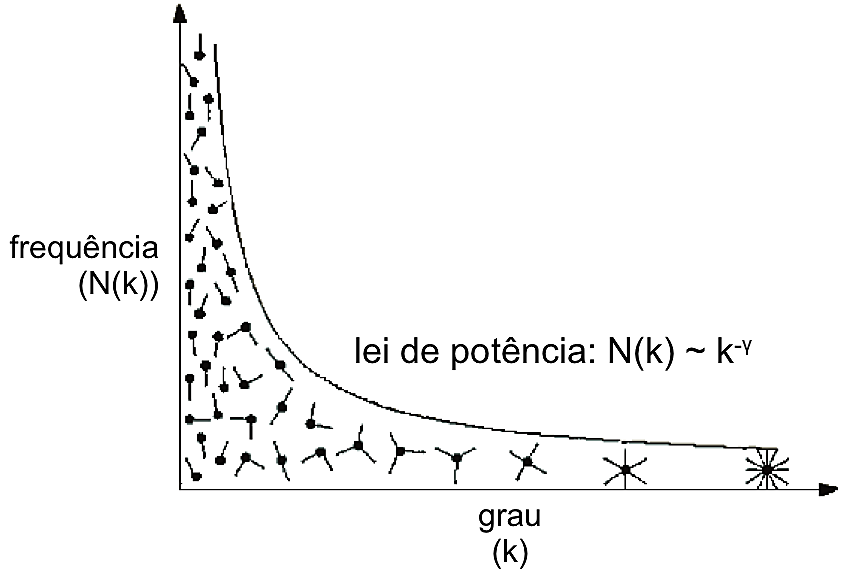
\includegraphics[width=0.6\textwidth]{figuras/leidepotencia}
	\caption{Distribuição do número de arestas por vértice do tipo lei de potência. Adaptado de \cite{Barabasi2007}.}
	\label{fig:leidepotencia}
\end{figure}

% No caso de redes orientadas, há duas distribuições a serem consideradas: a distribuição dos graus de entrada e a distribuição dos graus de saída. Nas redes orientadas que são livres de escala, ambas as distribuições seguem leis de potência.

% e alto coeficiente de clustering

Se diversas redes possuem um mesmo padrão de distribuição de graus, o que as diferencia? Milo e outros pesquisadores \cite{Milo2002} estudaram a estrutura de redes orientadas de diversos domínios em busca da resposta. Para isso, eles listaram 13 possíveis configurações de arestas em redes com 3 vértices --- as chamadas tríades ---, mostradas na Figura \ref{fig:triades}. Contando o número de vezes que cada tríade aparece em uma rede, é possível formar um vetor, denominado \emph{perfil de concentração de tríades} (PCT), que é característico de redes de um domínio. 

O papel dos PCTs na caracterização de domínios de redes é ilustrado nas Figuras \ref{fig:tcp}(a) e \ref{fig:tcp}(b). Na primeira Figura, são apresentados PCTs de redes de dois domínios distintos: uma rede de software e uma rede linguística. Na segunda, são apresentados PCTs de duas redes do mesmo domínio, o domínio de software. Uma análise informal dos gráficos revela que a similaridade entre os PCTs é maior no segundo caso, no qual as redes são do mesmo domínio. No primeiro caso, é notável a diferença nas concentrações das duas primeiras tríades (de cima para baixo). 
% 

\begin{figure}[htbp]
	\centering
		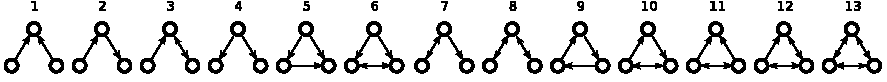
\includegraphics[scale=1]{figuras/triads}
	\caption{Tríades, ou grafos com três vértices, numeradas de 1 a 13.}
	\label{fig:triades}
\end{figure}

\begin{figure}[htbp]
	\centering
		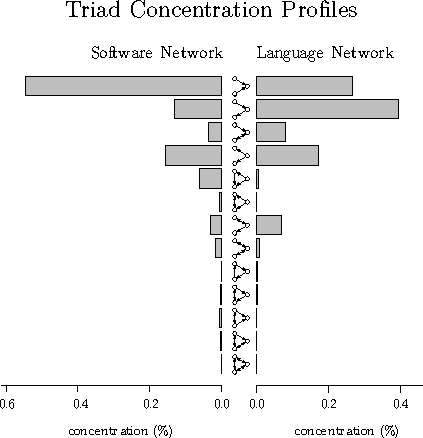
\includegraphics[width=1\textwidth]{figuras/tcp}
	\caption{Comparação entre perfis de concentração de tríades de três redes distintas. (a) À esquerda, rede de dependências entre as classes do programa JabRef, versão 2.5b2; à direita, rede de adjacências entre palavras da língua japonesa \cite{Milo2004}. (b) À esquerda, a rede do programa JabRef, versão 2.5b2; à direita, a rede do programa ArgoUML, versão 0.28.}
	\label{fig:tcp}
\end{figure}

A similaridade entre PCTs pode ser quantificada através do coeficiente de correlação de Pearson entre os PCTs \cite{Milo2004}. O resultado é um valor entre -1 (menor similaridade) e 1 (maior similaridade). Na Figura \ref{fig:tcp}(a), o coeficiente de correlação vale $0,68$; na Figura \ref{fig:tcp}(b), $0,98$. Os números confirmam a análise informal e mostram que a correlação é maior no caso em que as redes pertencem ao mesmo domínio.

Vale notar que o coeficiente de correlação neste caso não possui significado estatístico. Ainda assim, ele tem sido usado de forma bem sucedida na pesquisa de Milo.

A partir da similaridade entre PCTs pode-se construir uma métrica de similaridade entre redes. Sejam $a$ e $b$ duas redes, PCT($x$) o vetor com as concentrações das tríades na rede $x$ e cor($x, y$) o coeficiente de correlação de Pearson entre dois vetores. A similaridade entre as redes, sim($a$, $b$), é dada por:

$$
\mathrm{sim}(a, b) ~=~ 
  \mathrm{cor}(\mathrm{PCT}(a), \mathrm{PCT}(b))\mathrm{.}
$$

\end{section}

\begin{section}{Redes de Dependências no Domínio de Software}

	Redes são muito usadas no domínio de engenharia de software para representar as dependências entre entidades do código-fonte, tais como classes em linguagens orientadas a objetos. 
	%
	Estudos recentes têm aplicado a teoria das redes complexas a redes de dependências entre entidades do código-fonte de sistemas de software. 
	%
	(Daqui pra frente, tais redes serão denominadas \emph{redes de software}, em contraste com redes biológicas, redes sociais etc.) Um dos principais resultados é a constatação de que redes de software são livres de escala.
	%
	
	Valverde e Solé \cite{Valverde2003} estudaram redes não-orientadas formadas por relações de agregação de tipos em diagramas UML, programas em C e programas em C++. Myers \cite{Myers2003} analisou redes de chamadas de função em programas em C e redes de agregação e herança em programas em C++. Em ambos os casos as redes foram identificadas como livres de escala. 

	Redes livres de escala também foram encontradas em programas escritos em Smalltalk \cite{Marchesi2004,Concas2007} e em Java \cite{Hyland-Wood2006,Baxter2006,Ichii2008}, em dependências entre pacotes de software \cite{Labelle2004}, em dependências entre bibliotecas dinâmicas \cite{Louridas2008} e até mesmo em referências entre objetos em tempo de execução \cite{Potanin2005}.
\end{section}

\begin{section}{Modelos de Síntese de Redes Organizadas em Módulos}
% deu 7 páginas

Para tentar explicar os mecanismos responsáveis pela formação de redes livres de escala em diversos domínios, vários modelos de redes livres de escala foram propostos. Os modelos são algoritmos que geram vértices e arestas de forma probabilística porém de acordo com certas regras que garantem que, quando o número de vértices tende a infinito, a distribuição dos graus dos vértices tende a uma lei de potência. Tais modelos, portanto, geram redes similares a redes de software, ao menos quanto à distribuição dos graus.

Assim como um sistema de software é organizado conceitualmente em módulos, uma rede de software deve representar suas entidades organizadas em módulos. A maioria dos modelos de redes livres de escala, no entanto, gera redes sem qualquer tipo de organização hierárquica.

Após uma pesquisa extensa, embora não-sistemática, realizada durante o primeiro semestre de 2009, foram encontrados dois modelos de redes livres de escala organizadas em módulos: o modelo CGW \cite{Chen2008} e o modelo LFR \cite{Lancichinetti2008,Lancichinetti2009}. Um terceiro modelo, o BCR+, elaborado no contexto deste trabalho, é descrito no próximo capítulo.

% Modelo de Erdos-Renyi?
% Modelo de configuração?
% Modelo de Albert-Barabasi?

\begin{subsection}{O modelo CGW}

O modelo CGW \cite{Chen2008} foi proposto como um modelo da evolução de sistemas de software. O modelo aceita 11 parâmetros:

\begin{itemize}
\item número de vértices, $n$;
\item número de módulos, $m$;
\item quatro probabilidades, $p_1, p_2, p_3, p_4$, com $p_1 + p_2 + p_3 + p_4 = 1$ e $p_1 > 0$;
\item quatro números naturais, $e_1, e_2, e_3, e_4$;
\item uma constante, $\alpha$, com $\alpha \ge -1$.
\end{itemize}

Nesse modelo, a rede começa com poucos vértices e então vai crescendo de acordo com determinadas regras de formação, até alcançar $n$ vértices. Cada vértice pertence a um dos $m$ módulos.

Os autores do modelo CGW não deixam claro qual é a forma exata da rede inicial, e nem disponibilizam uma implementação do modelo. A implementação realizada nesta pesquisa considera que a rede inicial é formada por dois vértices contidos em um mesmo módulo, e uma aresta bidirecional que liga os vértices. A partir daí, a rede é alterada pela aplicação sucessiva de quatro regras em ordem aleatória:

\begin{itemize}
	
	\item Regra 1: com probabilidade $p_1$, um novo vértice é adicionado a um módulo escolhido aleatoriamente, juntamente com $e_1$ arestas com origem no novo vértice. Os vértices de destino das $e_1$ arestas são escolhidos de acordo com a probabilidade preferencial baseada em módulos (PPBM), explicada mais à frente.
	
	\item Regra 2: com probabilidade $p_2$, são adicionadas $e_2$ arestas. Para cada aresta, o vértice de origem é escolhido aleatoriamente, enquanto o vértice de destino é escolhido de acordo com a PPBM.
	
	\item Regra 3: com probabilidade $p_3$, $e_3$ arestas são religadas. O procedimento de religamento de arestas é descrito a seguir:
	
	\begin{enumerate}
		\item um vértice, $v_1$ é escolhido aleatoriamente;
		\item uma aresta, $a_1$, escolhida aleatoriamente dentre as arestas com origem em $v_1$, é removida da rede;
		\item é adicionada uma nova aresta cuja origem é $v_1$ e o vértice de destino é escolhido de acordo com a PPBM;
	\end{enumerate}
	
	\item Regra 4: com probabilidade $p_4$, $e_4$ arestas escolhidas aleatoriamente são removidas da rede.
	
\end{itemize}

Naturalmente, as probabilidades $p_1, p_2, p_3$ e $p_4$ devem somar 1. Além disso, $p_1$ deve ser maior que zero --- do contrário o número de vértices na rede permanece constante. As quantidades $e_1, e_2, e_3, $ e $e_4$ são inteiros maiores ou iguais a zero.

A probabilidade preferencial baseada em módulos, $\Pi(v_2|v_1)$, é uma função que indica a probabilidade de se escolher um vértice, $v_2$, como destino de uma aresta cujo vértice de origem, $v_1$, já foi determinado. O propósito da PPBM é controlar a proporção de arestas externas na rede, privilegiando a escolha de um vértice de destino pertencente ao mesmo módulo do vértice de origem (ou pertence a outro módulo, a depender do valor de $\alpha$). Eis a definição da probabilidade preferencial baseada em módulos:

$$
\Pi (v_2|v_1) ~=~
\left\{
\begin{array}{cl}
\dfrac{1 + \mathrm{g}(v_2) \cdot (1 + \alpha)}{Q(v_1)} 
  & \mbox{se $v_2$ está no mesmo módulo de $v_1$} \vspace{0.5em} \\ 
\dfrac{1 + \mathrm{g}(v_2)}{Q(v_1)} 
  & \mbox{caso contrário}
\end{array}
\right.
$$

O parâmetro $\alpha$ controla a proporção de arestas externas na rede. Para $\alpha = -1$, a maioria das arestas serão externas. Para $\alpha > 0$, a maioria das arestas serão internas, e quanto maior o valor de $\alpha$, maior a tendência. Quando $\alpha = 0$, arestas internas e externas são igualmente prováveis.

A expressão g($v$) designa o grau de saída do vértice $v$. O termo $Q$ é apenas uma constante de proporcionalidade cujo propósito é fazer a soma das probabilidades ser igual a 1, e é definido da seguinte forma:

$$
Q(v_1) = \sum_{v \in m(v_1)} (1 + \mathrm{g}(v) \cdot (1 + \alpha))
~+ \sum_{v \notin m(v_1)} (1 + \mathrm{g}(v))
$$

A expressão m($v$), neste contexto, designa o conjunto dos vértices que pertencem ao mesmo módulo de $v$.

\end{subsection}

\begin{subsection}{O modelo LFR}

O modelo LFR \cite{Lancichinetti2008,Lancichinetti2009} é um modelo flexível que pode gerar redes com arestas ponderadas e módulos sobrepostos, isto é, nas quais um vértice pode pertencer a mais de um módulo. Diferentemente do CGW, o LFR não é um modelo de crescimento: todos os vértices são gerados de uma vez e então são adicionadas as arestas.

Nesta pesquisa foi estudado um caso particular do modelo no qual todas as arestas têm o mesmo peso e os módulos não se sobrepõem. Foi usada a implementação original dos autores, disponível em  \url{http://santo.fortunato.googlepages.com/inthepress2}. O modelo aceita os seguintes parâmetros:

\begin{itemize}
\item número de vértices, $n$;
\item grau de entrada médio, $k$, com $k < n$;
\item grau de entrada máximo, $max_k$, com $k \le max_k < n$;
\item parâmetro de mistura, $\mu$, com $0 \le \mu \le 1$;
\item expoente da distribuição de graus, $-\gamma$;
\item expoente da distribuição de tamanho de módulos, $-\beta$;
\item tamanho do menor módulo, $min_m$;
\end{itemize}

Os tamanhos dos módulos são selecionados de uma lei de potência com expoente $-\beta$. O parâmetro de mistura, $\mu$, é a proporção de arestas externas na rede gerada. No modelo LFR, nem todas as combinações de parâmetros são factíveis. Por exemplo, se $n = 100$, então $min_m$ não pode ser 60, caso contrário existiriam módulos menores do que $min_m$.

\end{subsection}

\end{section}
% Avaliação da ("softwareness") Redes de Software e outros tipos de redes
% complexas (5-10)
%	
%		 * as redes geradas são verossímeis?
%
% deu 7 páginas.

\chapter{Avaliação de Modelos de Redes} \label{cap:avaliacao}

% TODO: explicar por que as redes de outros domínios são necessárias neste estudo.

\begin{section}{Introdução}
Os três modelos apresentados anteriormente --- BCR+, LFR e CGW --- geram redes que podem ser interpretadas como redes de software, contendo entidades de implementação organizadas em módulos e dependências entre as entidades. Para aumentar a confiança de que os resultados de estudos com redes sintéticas podem ser extrapolados para redes de software, no entanto, é preciso avaliar se, com uma escolha adequada de parâmetros, os modelos são capazes de gerar redes que se assemelham a redes de software. Daqui para frente, redes que se assemelham a redes de software serão chamadas de \emph{redes software-realistas}.

Já se sabe que os três modelos geram redes que, a exemplo de redes de software, são livres de escala. Isoladamente, no entanto, esta propriedade não é suficiente para avaliar os modelos, uma vez que muitas redes livres de escala conhecidas não são redes do software (por exemplo, redes biológicas). Partindo da hipótese de que redes de outros domínios são estruturalmente diferentes de redes de software, o critério usado para avaliar se as redes sintéticas são software-realistas deve ser robusto o suficiente para determinar que redes de outros domínios não são software-realistas.

Neste capítulo é descrito um experimento no qual se verificou que os três modelos geram redes software-realistas. A partir dessa conclusão, foi encontrado um subconjunto de valores para os parâmetros dos modelos que garantem, com alta taxa de acerto, que as redes geradas serão software-realistas.

A ideia básica do experimento é gerar redes usando diversos valores para os parâmetros dos modelos e então medir a similaridade entre as redes sintéticas e um conjunto de redes de software extraídas de sistemas reais e de redes de outros domínios. Para apoiar a realização do experimento, foram coletadas 131 redes:

\begin{itemize}
	\item redes de software: foram coletados 65 sistemas de software escritos em Java, contendo entre 111 e 35.563 classes cada um. A linguagem Java foi escolhida por ser uma linguagem de programação popular na qual muitos sistemas de software de código aberto já foram escritos. A maior parte dos sistemas foram selecionados a partir da lista dos sistemas mais populares do repositório SourceForge.net; além desses, foram selecionados sistemas com os quais o autor tem familiaridade, como o OurGrid. Para extrair a rede de dependências dos sistemas foi usada a ferramenta Dependency Finder, disponível em \url{http://depfind.sf.net/}, que foi escolhida pela facilidade de uso.
	\item redes de outros domínios: foram coletadas 66 redes de domínios tão diversos quanto a biologia, a sociologia, a tecnologia e a linguística, com tamanho variando entre 32 e 18.163 vértices.
\end{itemize}

\end{section}

\begin{section}{Software-realismo de uma Rede} \label{sec:realismo-rede}

Para apoiar o experimento, foi desenvolvido um modelo de classificação que classifica redes em dois grupos: software-realistas e não software-realistas. O modelo de classificação é baseado em uma métrica de similaridade entre duas redes. Para determinar a classificação de uma rede, é medida a similaridade da rede em relação a todas as 65 redes de software da amostra. A rede é considerada software-realista quando a média das similaridades é superior a um limiar pré-determinado.
	
Seguindo o trabalho de Milo et al. \cite{Milo2002}, cada rede é caracterizada pelo seu perfil de concentração de tríades (PCT), isto é, a frequência relativa de cada uma das treze tríades na rede. Seguindo outro trabalho de Milo et al. \cite{Milo2004}, a similaridade entre duas redes é medida a partir do cálculo do coeficiente de correlação de Pearson entre os PCTs das redes, que é um valor entre -1 (menor similaridade) e 1 (maior similaridade):

$$
\mathrm{sim}(a, b) ~=~ 
  \mathrm{cor}(\mathrm{PCT}(a), \mathrm{PCT}(b))\mathrm{,}
$$

onde $a$ e $b$ são redes, PCT($x$) é um vetor com as concentrações das tríades na rede $x$ e cor($x, y$) é o coeficiente de correlação de Pearson entre dois vetores.

Vale notar que o coeficiente de correlação neste caso não possui significado estatístico. Ainda assim, ele têm sido usado de forma bem sucedida na pesquisa de Milo e, como será mostrado a seguir, rendeu bons resultados nesta pesquisa.

A partir da métrica de similaridade entre redes, foi desenvolvida a métrica S, que representa o quanto uma rede se assemelha a redes de software. O valor de S para uma rede $x$, S($x$), é definido como a similaridade média entre a rede $x$ e uma amostra de redes de software, $R$:

$$
\mathrm{S}(x) ~=~ \frac{
\displaystyle\sum_{s \in R} \mathrm{sim}(x, s)
}{|R|} \mathrm{,}
$$

Neste estudo, consideramos que $R$ é a amostra de 65 redes de software.

Para os propósitos desta pesquisa, a métrica S deve satisfazer duas condições: (i) ela deve ter valores altos quando aplicada a redes de software; (ii) ela deve ter valores mais baixos quando aplicadas a redes de outros domínios. Com a finalidade de avaliar se a métrica satisfaz as condições, foi computada métrica S de cada uma das 131 redes selecionadas para este estudo. Para a extração dos PCT, foi usada a ferramenta igraph \cite{igraph}.

O valor de S para as redes de software oscilou entre 0,83 e 0,98, com média igual a 0,97 e desvio-padrão igual a 0,03. O alto valor médio de S e o baixo desvio-padrão mostra que a métrica caracteriza adequadamente as redes de software, capturando seus padrões estruturais.

Um total de 97,0\% das redes de outros domínios recebeu um valor de S inferior a 0,83. Algumas redes receberam valores negativos de S, revelando uma alta dissimilaridade com redes de software. Apenas duas redes receberam valores altos de S: a rede de links entre blogs sobre política (S = 0,97) e a rede neural do verme C. Elegans (S = 0,88). Investigações futuras serão necessárias para descobrir as razões por trás dos valores altos e métricas auxiliares que possam diferenciar as duas redes de redes de software.

A partir da métrica S é definido um modelo de classificação de redes: redes com valor S superiores a um determinado limiar são classificadas como redes software-realistas; as demais redes são classificadas como não software-realistas.

Como existem redes de outros domínios com valor de S alto, é impossível construir um modelo de classificação perfeito, independentemente da escolha do limiar. Um modelo de classificação pode, no entanto, ser avaliado em termos de sua precisão e de sua cobertura. Seja $R$ o conjunto de 65 redes de software e $L$ o subconjunto das 131 redes que são classificadas como software-realistas. A precisão do modelo é

$$
\mbox{precisão}: ~\frac{R \cap L}{L},
$$

e a cobertura é

$$
\mbox{cobertura}: ~\frac{R \cap L}{R}.
$$

Aumentar o limiar tem o efeito de reduzir a cobertura, pelo fato de menos redes de software serem classificadas como software-realistas. Reduzir o limiar tem o efeito de reduzir a precisão, pelo fato de mais redes de outros domínios serem classificadas como software-realistas.

A escolha de um limiar adequado, portanto, depende da importância dada à precisão e à cobertura. Como o objetivo do experimento é avaliar se redes sintéticas são software-realistas, é mais importante ter alta precisão, pois isso representa um teste mais forte.

Para obter 100\% de precisão, o limiar deve ser 0,98, um valor que está acima do maior valor de S para redes de outros domínios. A cobertura, neste caso, seria de apenas 44,6\%, pois muitas redes de software seriam incorretamente classificadas. Foi escolhido o valor 0,88 para o limiar, que é suficiente para classificar a rede do verme C. Elegans como não software-realista e render valores altos para a cobertura (95,4\%) e para a precisão (96,9\%).

\end{section}

\begin{section}{Avaliação Empírica do Software-realismo de Modelos de Redes}

Na seção anterior foi mostrado que muitas redes livres de escala de diversos domínios podem ser diferenciadas de redes de software através de um modelo de classificação simples baseado em perfis de concentração de tríades (PCTs). Nessa seção é descrito um experimento que mostra que os três modelos de redes organizadas em módulos geram redes software-realistas. O experimento consiste em gerar redes usando diversas combinações de parâmetros dos três modelos, e então classificar cada rede como software-realista ou não software-realista. O número de vértices foi fixado em 1.000 e os valores dos demais parâmetros foram variados em passos discretos. No total, foram geradas 9.500 redes com o modelo BCR+, 38.790 redes com o modelo CGW e 1.296 redes com o modelo LFR.

\begin{subsection}{Seleção de Parâmetros} \label{sec:parametros}

Para o modelo BCR+, foram escolhidos grafos de módulos extraídos a partir de dependências entre arquivos JAR de 5 sistemas de software: GEF (2 módulos), iBATIS (4 módulos), MegaMek (8 módulos), findbugs (16 módulos) e zk (32 módulos). Como muitos dos arquivos JAR foram concebidos para serem reusados em projetos distintos, eles são uma boa aproximação do conceito de módulo. Para os demais parâmetros, os seguintes valores foram escolhidos:

\begin{itemize}
	\item $p_1, p_2, p_3 \in \{0,0; 0,2; 0,4; 0,6; 0,8; 1,0\}$, com $p_1 + p_2 + p_3 = 1$ e $p_1 + p_2 > 0$ (do contrário a rede jamais alcançaria 1.000 vértices);
	\item $\delta_{in}, \delta_{out} \in \{0, 1, 2, 3, 4\}$;
	\item $\mu \in \{0,0; 0,2; 0,4; 0,6\}$ (valores altos foram evitados a fim de ignorar redes com módulos fortemente acoplados).
\end{itemize}

Para o modelo CGW, os seguintes valores de parâmetros foram escolhidos:

\begin{itemize}
	\item $p_1, p_2, p_3, p_4 \in \{0,0; 0,2; 0,4; 0,6; 0,8; 1,0\}$, com $p_1 + p_2 + p_3 + p_4 = 1$ e $p_1 > 0$ (do contrário a rede jamais alcançaria 1000 vértices);
	\item $e_1, e_2, e_3, e_4 \in \{1, 2, 4, 8\}$ (com a restrição de que $e_i$ não varia quando $p_i = 0$, o que não faria sentido);
	\item $\alpha \in \{-1, 0, 1, 10, 100, 1000\}$
	\item $m \in \{2, 4, 8, 16, 32\}$.
\end{itemize}

No caso do modelo LFR, os seguintes valores foram escolhidos para os parâmetros:

\begin{itemize}
	\item parâmetro de mistura: $\mu \in \{0,0; 0,2; 0,4; 0,6\}$;
	\item expoente da distribuição de graus: $\gamma \in \{2,18; 2,70; 3,35\}$;
	\item expoente da distribuição de tamanhos de módulos: $\beta \in \{0,76; 0,99; 1,58\}$;
	\item grau médio: $k \in \{5, 10, 15, 25\}$;
	\item grau máximo: $max_k \in \{58, 157, 482\}$;
	\item tamanho do menor módulo: $min_m \in \{1, 10, 273\}$.
\end{itemize}

Para chegar aos valores para os parâmetros do modelo LFR, foram analisadas métricas de redes de software com cerca de 500 a 2.000 classes. Para cada métrica foram identificados os valores mínimo, mediano e máximo; esses foram os valores usados nos parâmetros correspondentes.
\end{subsection}

\begin{subsection}{Resultados}

Usando o modelo de classificação descrito na Seção \ref{sec:realismo-rede}, cada rede sintética foi classificada como software-realista ou não software-realista. Os resultados estão condensados na Tabela \ref{tab:results}.

\begin{table}
\caption{Resultados da classificação de redes sintéticas}
\centering
\begin{tabular}{|l|l|}
\hline
Model & Networks classified as software-like \\
\hline 
\hline
BCR+ & 21.18\% \\ % 2012 / 9500
\hline
CGW  & 19.40\% \\  % 7524 / 38790
\hline
LFR  & 31.25\% \\ %  405 / 1296
\hline
\end{tabular}
\label{tab:results}
\end{table}

Todos os modelos geraram redes software-realista e redes não software-realistas. A proporção de redes software-realistas foi maior que 19\% em todos os casos, descartando a possibilidade de que esse resultado tenha sido obtido por acaso. (A proporção exata para cada modelo não deve ser não deve ser interpretada como medida de qualidade, pois com esses resultados não é possível determinar se um modelo é melhor do que os outros.)
% Para afirmar isso seria necessário repetir o experimento com redes de Erdos-Renyi

Naturalmente, esse resultado tem pouco valor prático se não for estabelecido uma relação entre os valores dos parâmetros usados na geração de uma rede e a classificação da rede. Na prática é importante saber quais valores de parâmetros tendem a gerar redes software-realistas.

Para ajudar a descobrir essa relação, foi utilizado o algoritmo 1R \cite{OneR} da mineração de dados. O algoritmo analisa, para cada rede, os parâmetros usados na sua geração e a sua classificação, e então encontra uma regra que relaciona o valor de um único parâmetro com a classificação da rede. Regras encontradas pelo 1R podem ser avaliadas de acordo com a sua acurácia, isto é, a proporção de redes corretamente classificadas.

As regras encontradas pelo algoritmo 1R são exibidas na Tabela \ref{tab:rules}. As regras são bastante simples e, portanto, fáceis de seguir. (Essa característica do 1R foi o que motivou a sua escolha em detrimento de outros algoritmos de mineração de dados.) Apesar da simplicidade, as regras encontradas possuem uma acurácia de cerca de 80\% para todos os modelos.

\begin{table}
\caption{Regras para prever a classificação de uma rede sintética.}
\centering
\begin{tabular}{|l|l|l|}
\hline
Modelo & Regra & Acurácia \\
\hline 
\hline
\multirow{2}{*}{BCR+}
     & $p_1 \ge 0.7 \Rightarrow \mbox{rede software-realista}$ & \multirow{2}{*}{82.4\%}  \\ 
     & $p_1 < 0.7 \Rightarrow \mbox{rede não software-realista}$ & \\ 
\hline
\multirow{2}{*}{CGW}
     & $p_1 \ge 0.5 \Rightarrow \mbox{rede software-realista}$ & \multirow{2}{*}{82.3\%} \\  
     & $p_1 < 0.5 \Rightarrow \mbox{rede não software-realista}$ & \\  
\hline
\multirow{2}{*}{LFR}   
     & $\gamma < 2.44 \Rightarrow \mbox{rede software-realista}$ & \multirow{2}{*}{78.9\%} \\ 
     & $\gamma \ge 2.44 \Rightarrow \mbox{rede não software-realista}$ & \\ 
\hline
\end{tabular}
\label{tab:rules}
\end{table}

\end{subsection}

\end{section}


 
% Descrição do experimento segundo o arcabouço de Basili.
% 
% Descrição geral do experimento: similaridade entre redes sintéticas e redes de software usando tríades.
% 
% PARTE 1
% 
% Similaridade entre duas redes.
% 
% Conjuntos de dados.
% 
% Métrica de softwareness e avaliação através de precisão e cobertura.
% 
% PARTE 2
% 
% Avaliação dos modelos
% 
% Escolha dos parâmetros
% 
% Resultados
% (5-20)

\chapter{Estudo sobre Algoritmos de Agrupamento} \label{cap:estudo}

Caracterização do experimento segundo framework de Basili.

Objetivos (perguntas a responder):
1. ...
2. ...

Método:
Design fatorial

..
..
..

Resultados:

..
 
% 2-10 páginas

%   (Limitações)
%   (Lições aprendidas)
% Recapitulação
% Resumo das contribuições
% Trabalhos futuros

\chapter{Conclusão} \label{cap:conclusao}

Neste trabalho foi apresentada uma nova abordagem para avaliação de algoritmos de agrupamento de software, baseada na simulação de modelos de redes organizadas em módulos. Mostrou-se, através de um experimento, que pelo menos três modelos de redes são capazes de gerar redes que se assemelham a redes de dependências estáticas entre classes em programas orientados a objetos. A partir deste resultado, foi feito um estudo sobre algoritmos de agrupamento de software usando a abordagem apresentada no trabalho.

Este trabalho não diminui a importância de se avaliar algoritmos de agrupamento usando redes extraídas de sistemas de software reais analisadas por especialistas humanos. Ainda assim, o uso de redes de software sintéticas de forma complementar pode ser vantajoso no estudo dos algoritmos. Primeiramente, o uso de modelos permite a criação de conjuntos de teste extensos. Além disso, as redes são criadas de maneira controlada, de acordo com parâmetros pré-definidos, o que torna possível estudar o comportamento dos algoritmos com diversos valores de parâmetros.

O uso de conjuntos de dados sintéticos, produzidos por modelos, é comum na pesquisa de sistemas distribuídos e redes, mas ainda pouco explorado na pesquisa de engenharia de software. O impacto deste trabalho pode ir além da comunidade de agrupamento de software, uma vez que muitas tarefas de engenharia reversa usam dependências entre entidades de software para extrair informações sobre sistemas.

As contribuições desta pesquisa para o estado da arte podem ser assim resumidas:

\begin{itemize}
	\item identificação de dois modelos de redes organizadas em módulos, CGW e LFR, adequados para o teste de algoritmos de agrupamento;
	\item adaptação de um modelo de redes, o BCR, para produzir redes organizadas em módulos;
	\item fornecimento de evidências empíricas de que certos modelos geram redes software-realistas, isto é, redes que se assemelham a redes extraídas de sistemas de software;
	\item identificação de valores para os parâmetros dos três modelos que induzem a geração de redes software-realistas;
	\item comparação do desempenho de quatro algoritmos de agrupamento de software: ACDC, Bunch, SL e CL;
	\item entendimento da variação do número de módulos de uma rede no desempenho dos algoritmos de agrupamento.
\end{itemize}

As quatro primeiras contribuições desta pesquisa foram documentadas no artigo ``Modular Network Models for Class Dependencies in Software'', aceito para publicação no 14º Congresso Europeu sobre Manutenção de Software e Reengenharia (CSMR 2010). Há planos de escrever um outro artigo com os resultados completos da pesquisa.

%%% LIMITAÇÕES

Naturalmente, este trabalho possui algumas limitações que poderão ser endereçadas em trabalhos futuros. A representação usada para sistemas de software --- grafo orientado --- é bastante simples e abstrai aspectos de sistemas de software que podem ser importantes, como a diferenciação de tipos de entidades (classes, atributos, métodos, arquivos fonte etc.). Além disso, o grafo orientado não diferencia diversos tipos de relacionamento entre entidades, como chamada de método, leitura de atributo etc. Em vez disso, todos os relacionamentos são abstraídos sob a forma do relacionamento de dependência.

O foco deste trabalho foi o agrupamento de entidades de software em módulos de forma a minimizar dependências entre módulos. Existem, no entanto, outros critérios para agrupar entidades de software. Por exemplo, algumas pesquisas se preocupam em estudar o agrupamento de entidades que implementam funcionalidades relacionadas. Os modelos estudados neste trabalho não incorporam o conceito de funcionalidade e, portanto, não são adequados para se estudar agrupamentos de entidades de software sob o ponto de vista funcional.

% Limitações
% 
% Trabalhos futuros
%   Refinar modelos, com informações hierárquicas, tipos de vértices, múltiplas arestas com tipos e peso...
%   Refinar modelos, adicionando a dimensão da evolução
%   Pesquisar outros problemas, além de clustering de software, que possam se beneficiar de modelos baseados nos modelos aqui apresentados.

%%%%%%%%%%%%%%%%%%%%%%%%%%%%%%%%%%%%%%%%%%%%%%%%%%%%%%%%%%%%%%%%%%%%%%%%%%%%%%
%% BIbliografia
%% Coloque suas referencias no arquivo ref.bib e descomente as proximas duas linhas

\bibliographystyle{plain} % estilo de bibliografia   plain,unsrt,alpha,abbrv.
\bibliography{ref} % arquivos com as entradas bib.

%%%%%%%%%%%%%%%%%%%%%%%%%%%%%%%%%%%%%%%%%%%%%%%%%%%%%%%%%%%%%%%%%%%%%%%%%%%%%%%%
%% Apendice
% Caso seja necessario algum apendice, descomente a proxima linha.

\appendix
\begin{chapter}{Redes Empregadas na Avaliação dos Modelos} \label{cap:lista-redes}
% select nme_network, to_char(s_score, '0.99'), n_vertices, n_edges 
% from view_network
% where fk_classification = 1
% OR nme_network ilike '%irpf%'
%

\begin{center}
\begin{longtable}{| p{10cm} | c | r | r |}
	\caption{65 redes de software (conjunto $T$).}	\\
	\hline
	\textbf{Sistema} & \textbf{S($x$, $T$)} & \textbf{Vértices} & \textbf{Arestas} \\ \hline
	\hline
	% AbaGuiBuilder-1.8 &  $0,97$ & 2929 & 12399 \\ \hline
	% alfresco-labs-deployment-3Stable &  $0,97$ & 2441 & 9178 \\ \hline
	% aoi272 &  $0,98$ & 1579 & 11670 \\ \hline
	% ArgoUML-0.28 &  $0,97$ & 5075 & 29018 \\ \hline
	% battlefieldjava-0.1 &  $0,98$ & 707 & 2038 \\ \hline
	% broker-4.1.5 &  $0,97$ & 5940 & 25589 \\ \hline
	% checkstyle-5.0 &  $0,98$ & 1174 & 4513 \\ \hline
	% dbwrench &  $0,98$ & 2015 & 10188 \\ \hline
	% dom4j-1.6.1 &  $0,98$ & 4666 & 31689 \\ \hline
	% ec2-api-tools &  $0,98$ & 5255 & 26916 \\ \hline
	% ermodeller-1.9.2-binary &  $0,97$ & 1441 & 6261 \\ \hline
	% findbugs-1.3.8 &  $0,98$ & 3401 & 20023 \\ \hline
	% flyingsaucer-R8 &  $0,97$ & 1323 & 6610 \\ \hline
	% freetts-1.2.2-bin &  $0,91$ & 273 & 1106 \\ \hline
	% ganttproject-2.0.9 &  $0,98$ & 5447 & 25558 \\ \hline
	% gdata-src.java-1.31.1 &  $0,97$ & 1649 & 8150 \\ \hline
	% GEF-0.13-bin &  $0,97$ & 352 & 1484 \\ \hline
	% geoserver-2.0-beta1-bin &  $0,97$ & 25007 & 145034 \\ \hline
	% geotools-2.5.5-bin &  $0,97$ & 13559 & 79499 \\ \hline
	% gfp\_0.8.1 &  $0,87$ & 475 & 1030 \\ \hline
	% guice-2.0 &  $0,98$ & 638 & 2980 \\ \hline
	% gwt-windows-1.6.4 &  $0,98$ & 6065 & 32729 \\ \hline
	% hibernate-distribution-3.3.1.GA-dist &  $0,98$ & 4340 & 22410 \\ \hline
	% Hl7Comm.1.0.1 &  $0,97$ & 337 & 1335 \\ \hline
	% hsqldb\_1\_8\_0\_10 &  $0,95$ & 369 & 1901 \\ \hline
	% iBATIS\_DBL-2.1.5.582 &  $0,95$ & 291 & 1300 \\ \hline
	% iFreeBudget-2.0.9 &  $0,98$ & 4053 & 20028 \\ \hline
	% iReport-nb-3.5.1 &  $0,97$ & 35019 & 184701 \\ \hline
	% IRPF2009v1.1 &  $0,98$ & 5396 & 29247 \\ \hline
	% JabRef-2.5b2-src &  $0,98$ & 2473 & 10437 \\ \hline
	% jai-1\_1\_4-pre-dr-b03-lib-linux-i586 &  $0,96$ & 936 & 5086 \\ \hline
	% jailer\_2.9.9 &  $0,97$ & 3691 & 14890 \\ \hline
	% jakarta-tomcat-5.0.28-embed &  $0,98$ & 2314 & 10652 \\ \hline
	% jalopy-1.5rc3 &  $0,98$ & 888 & 4349 \\ \hline
	% jasperreports-3.5.2-project &  $0,98$ & 20508 & 120243 \\ \hline
	% jfreechart-1.0.13 &  $0,97$ & 1989 & 13891 \\ \hline
	% jGnash-2.2.0 &  $0,98$ & 6948 & 38303 \\ \hline
	% jgraphpad-5.10.0.2 &  $0,96$ & 519 & 2257 \\ \hline
	% jmsn-0.9.9b2 &  $0,83$ & 232 & 777 \\ \hline
	% juel-2.1.2 &  $0,94$ & 111 & 435 \\ \hline
	% juxy-0.8 &  $0,97$ & 3025 & 20427 \\ \hline
	% JXv3.2rc2deploy &  $0,96$ & 711 & 2573 \\ \hline
	% makagiga-3.4 &  $0,98$ & 1999 & 10819 \\ \hline
	% MegaMek-v0.34.3 &  $0,98$ & 2855 & 19575 \\ \hline
	% mondrian-3.1.1.12687 &  $0,97$ & 2000 & 14128 \\ \hline
	% myjgui\_0.6.6 &  $0,96$ & 604 & 2430 \\ \hline
	% oddjob-0.26.0 &  $0,98$ & 4204 & 18752 \\ \hline
	% openxava-3.1.2 &  $0,98$ & 16919 & 89049 \\ \hline
	% pdfsam-1.1.3-out &  $0,97$ & 3043 & 16024 \\ \hline
	% peer-4.1.5 &  $0,97$ & 9291 & 50614 \\ \hline
	% pentaho-reporting-engine-classic-0.8.9.11 &  $0,98$ & 3454 & 17948 \\ \hline
	% pjirc\_2\_2\_1\_bin &  $0,84$ & 180 & 687 \\ \hline
	% pmd-bin-4.2.5 &  $0,98$ & 1719 & 8098 \\ \hline
	% proguard4.3 &  $0,98$ & 604 & 4923 \\ \hline
	% rapidminer-4.4-community &  $0,96$ & 11764 & 55976 \\ \hline
	% smc\_6\_0\_0 &  $0,97$ & 698 & 3571 \\ \hline
	% squirrel-sql-3.0.1-base &  $0,98$ & 8982 & 43806 \\ \hline
	% squirrel-sql-3.0.1-standard &  $0,98$ & 11922 & 53969 \\ \hline
	% stendhal-0.74 &  $0,97$ & 747 & 3056 \\ \hline
	% subethasmtp-3.1 &  $0,98$ & 1485 & 8174 \\ \hline
	% thinkui\_sqlclient-1.1.2 &  $0,97$ & 2883 & 21979 \\ \hline
	% tvbrowser-2.7.3-bin &  $0,97$ & 3335 & 14110 \\ \hline
	% villonanny-2.3.0.b02.bin &  $0,98$ & 1949 & 6708 \\ \hline
	% worker-4.1.5 &  $0,97$ & 5940 & 25589 \\ \hline
	% zk-bin-3.6.1 &  $0,95$ & 13911 & 82219 \\ \hline
	
	abaguibuilder-1.8 & 0,94 & 875 & 3695 \\ \hline
	alfresco-labs-deployment-3Stable & 0,82 & 134 & 271 \\ \hline
	argouml-0.28 & 0,93 & 2436 & 12505 \\ \hline
	ArtOfIllusion272 & 0,96 & 1041 & 8597 \\ \hline
	battlefieldjava-0.1 & 0,63 & 98 & 320 \\ \hline
	checkstyle-5.0 & 0,93 & 349 & 1084 \\ \hline
	dbwrench & 0,97 & 1061 & 6732 \\ \hline
	dom4j-1.6.1 & 0,96 & 190 & 903 \\ \hline
	ec2-api-tools-1.3-36506 & 0,28 & 321 & 1023 \\ \hline
	findbugs-1.3.8 & 0,96 & 1581 & 8857 \\ \hline
	flyingsaucer-R8 & 0,92 & 536 & 2540 \\ \hline
	fm & 0,95 & 508 & 1889 \\ \hline
	freetts-1.2.2-bin & 0,89 & 113 & 399 \\ \hline
	ganttproject-2.0.9 & 0,96 & 1050 & 5177 \\ \hline
	gdata & 0,94 & 1194 & 6926 \\ \hline
	GEF-0.13-bin & 0,95 & 336 & 1387 \\ \hline
	geotools-2.5.5 & 0,95 & 6433 & 40651 \\ \hline
	GFP & 0,85 & 418 & 889 \\ \hline
	groovy-all-1.5.5 & 0,95 & 1537 & 7733 \\ \hline
	guice-2.0 & 0,96 & 639 & 3123 \\ \hline
	gwt-windows-1.6.4 & 0,97 & 6076 & 32801 \\ \hline
	hibernate-distribution-3.3.1.GA & 0,96 & 1711 & 10157 \\ \hline
	Hl7Comm.1.0.1 & 0,09 & 63 & 123 \\ \hline
	hsqldb & 0,94 & 309 & 1763 \\ \hline
	iBATIS\_DBL-2.1.5.582 & 0,94 & 279 & 1267 \\ \hline
	iReport-nb-3.5.1 & 0,94 & 2475 & 7068 \\ \hline
	jacorb & 0,92 & 4346 & 38844 \\ \hline
	jai-1\_1\_4-pre-dr-b03-lib-linux-i586-08\_Jun\_2009 & 0,94 & 936 & 5086 \\ \hline
	jailer & 0,87 & 328 & 1142 \\ \hline
	jalopy-1.5rc3 & 0,96 & 647 & 3460 \\ \hline
	jasperreports-3.5.2 & 0,97 & 1522 & 9080 \\ \hline
	jaxb & 0,96 & 2280 & 14298 \\ \hline
	jboss-5.1.0.GA & 0,97 & 4284 & 18360 \\ \hline
	jfreechart-1.0.13 & 0,95 & 1010 & 7663 \\ \hline
	jGnash & 0,96 & 765 & 3513 \\ \hline
	jgraphpad-5.10.0.2 & 0,95 & 519 & 2257 \\ \hline
	jmsn-0.9.9b2 & 0,84 & 232 & 777 \\ \hline
	jruby & 0,92 & 4714 & 33891 \\ \hline
	juel-2.1.2 & 0,92 & 111 & 437 \\ \hline
	juxy-0.8 & 0,87 & 77 & 198 \\ \hline
	jxplorer & 0,96 & 394 & 1511 \\ \hline
	makagiga-3.4 & 0,96 & 1981 & 10873 \\ \hline
	MegaMek-v0.34.3 & 0,96 & 1787 & 11245 \\ \hline
	mondrian-3.1.1.12687 & 0,94 & 1716 & 12035 \\ \hline
	myjgui\_0.6.6 & 0,9 & 127 & 419 \\ \hline
	oddjob-0.26.0 & 0,95 & 1208 & 5966 \\ \hline
	openide & 0,95 & 1421 & 6545 \\ \hline
	ourgrid-4.1.5 & 0,72 & 855 & 3218 \\ \hline
	pdfsam-1.1.3-out & 0,96 & 205 & 770 \\ \hline
	pentaho-reporting-engine-classic-0.8.9.11 & 0,96 & 1219 & 5727 \\ \hline
	pjirc\_2\_2\_1\_bin & 0,83 & 180 & 687 \\ \hline
	pmd-4.2.5 & 0,92 & 723 & 3828 \\ \hline
	proguard4.3 & 0,96 & 604 & 4923 \\ \hline
	rapidminer-4.4 & 0,93 & 2648 & 15096 \\ \hline
	richfaces-ui-3.3.0.GA & 0,95 & 865 & 1432 \\ \hline
	smc\_6\_0\_0 & 0,95 & 148 & 1249 \\ \hline
	squirrel-sql-3.0.1-base & 0,96 & 1171 & 4262 \\ \hline
	stendhal-0.74 & 0,95 & 468 & 1513 \\ \hline
	subethasmtp-3.1 & 0,85 & 85 & 217 \\ \hline
	thinkui\_sqlclient-1.1.2 & 0,96 & 944 & 7563 \\ \hline
	tvbrowser-2.7.3 & 0,96 & 3335 & 14133 \\ \hline
	VilloNanny & 0,96 & 100 & 585 \\ \hline
	weka & 0,92 & 2165 & 12834 \\ \hline
	xalan & 0,94 & 1439 & 10413 \\ \hline
	zk-bin-3.6.1 & 0,95 & 1753 & 8360 \\ \hline
	
	% \caption{\label{tab:redes}Sistemas de software usados no estudo de software-realismo de modelos e respectivos valores S.}
\end{longtable}
\end{center}


\begin{center}
\begin{longtable}{| p{6cm} | l | r | r | }
	\caption{66 redes de domínios diversos (conjunto $\bar{T}$).} \\
	\hline
	\textbf{Rede} & \textbf{S($x$, $T$)} & \textbf{Vértices} & \textbf{Arestas} \\ \hline
	\hline
	5 redes de amizade do site Facebook \cite{Traud2008} & $-0,130 \pm 0,007$ & 768 a 18162 & 33312 a 1533600 \\ \hline
	3 redes de circuitos eletrônicos \cite{Milo2004} & $0,433 \pm 0,005$ & 121 a 511 & 189 a 819 \\ \hline
	4 redes de adjacências entre palavras \cite{Milo2004} & $0,573 \pm 0,064$ & 2703 a 11585 & 8300 a 46281 \\ \hline
	3 redes de estrutura proteica \cite{Milo2004} & $0,540 \pm 0,046$ & 52 a 96 & 123 a 213 \\ \hline
	2 redes sociais de sentimento positivo \cite{Milo2004} & $0,555 \pm 0,248$ & 31 a 66 & 96 a 182 \\ \hline
	43 redes metabólicas \cite{Jeong2000} & $0,509 \pm 0,015$ & 408 a 2360 & 792 a 5959 \\ \hline
	Rede de interação entre proteínas da levedura \cite{Jeong2001} & $0,22$ & 687 & 1079 \\ \hline
	Links entre blogs políticos \cite{Adamic2005} & $0,96$ & 1489 & 19090 \\ \hline
	Rede neural do verme C Elegans \cite{Watts1998} & $0,87$ & 296 & 2359 \\ \hline
	Rede ``beta3sreduced'' (fonte desconhecida) & $0,05$ & 1286 & 33813 \\ \hline
	Rede ``czech'' (fonte desconhecida) & $0,78$ & 5225 & 51687 \\  \hline
	Rede ``ecoli-metabolic'' (fonte desconhecida) & $0,69$ & 895 & 964 \\ \hline
	
	% \caption{\label{tab:redes-outros}Redes de domínios diversos usados no estudo de software-realismo de modelos e respectivos valores S.}
\end{longtable}
\end{center}

\end{chapter}

\begin{chapter}{Algoritmos de Agrupamento} \label{cap:agrupamento}

A seguir são descritos brevemente três tipos de algoritmos de agrupamento de software que operam sobre redes de dependências entre entidades. % Para esta pesquisa foram escolhidos algoritmos estudados por diferentes grupos de pesquisa e com implementações disponíveis publicamente.

\begin{section}{Algoritmos Hierárquicos Aglomerativos}

Algoritmos hierárquicos aglomerativos têm sido aplicados a diversos problemas, incluindo o agrupamento de software \cite{Anquetil1999,Maqbool2007}. Essa família de algoritmos funciona com qualquer descrição de entidade, desde que seja fornecida uma métrica de similaridade entre pares de entidades. A similaridade entre duas entidades é medida em uma escala contínua de 0 a 1. O algoritmo é simples: inicia-se com um módulo para cada entidade e então mesclam-se sucessivamente os dois módulos mais similares até restar apenas um módulo com todas as entidades.

No contexto de recuperação de arquitetura de software, é comum descrever as entidades de código-fonte como um grafo de dependências entre entidades e usar a métrica de Jaccard para medir a similaridade entre duas entidades \cite{Anquetil1999}. Sejam X e Y duas entidades, e seja d(A) o conjunto de entidades ligadas à entidade A no grafo de dependências. A similaridade entre duas entidades, X e Y, é dada pela expressão a seguir:

$$
\mathrm{sim}(X, Y) ~=~ \frac{|\mathrm{d}(X) \cap \mathrm{d}(Y)|}{|\mathrm{d}(X) \cup \mathrm{d}(Y)|}
$$

O que diferencia os algoritmos hierárquicos aglomerativos entre si é o critério usado para medir a similaridade entre dois módulos. Os dois critérios mais estudados no contexto de agrupamento são chamados de ligação simples (SL, do inglês \emph{single linkage}) e ligação completa (CL, do inglês \emph{complete linkage}). Na ligação simples, a similaridade entre dois módulos é computada como a maior similaridade entre pares de entidades tiradas uma de cada módulo. Na ligação completa é considerada a menor similaridade.

Naturalmente, um agrupamento que consiste de apenas um módulo com todas as entidades analisadas é de pouco valor. Por essa razão deve existir um critério de parada que interrompa o algoritmo antes de todos os módulos terem sido mesclados em um grande módulo. No contexto de agrupamento de software, o critério mais comumente usado é a altura de corte, $h$, que varia entre 0 e 1. Sob esse critério, o algoritmo interrompe sua execução quando a maior similaridade entre dois módulos é menor ou igual a $1 - h$. Assim, quanto maior a altura de corte $h$, menor o número de módulos do agrupamento resultante.
	
\end{section}

\begin{section}{Bunch}

Com a finalidade de auxiliar a compreensão de programas, o algoritmo Bunch \cite{Mancoridis1998} agrupa o conjunto de entidades de um programa de acordo com os relacionamentos existentes entre elas, representados como um grafo orientado. O agrupamento é tratado como um problema de otimização no qual o objetivo é maximizar uma função denominada qualidade de modularização (QM), que recompensa agrupamentos com muitas arestas internas (que ligam entidades de um mesmo módulo) e poucas arestas externas (que ligam entidades de módulos distintos).

Encontrar um agrupamento que possui QM ótima é um problema intratável; por isso o algoritmo Bunch usa heurísticas como algoritmos genéticos e \emph{hill-climbing} para obter resultados quase ótimos.

\end{section}

\begin{section}{ACDC}

O algoritmo ACDC \cite{Tzerpos2000} foi projetado com o intuito de encontrar agrupamentos que facilitam a compreensão de programas. Assim como o Bunch, ele opera sobre grafos orientados. Sua principal característica é a identificação de conjuntos dominantes de vértices no grafo. Um conjunto dominante é um conjunto de vértices, $v_0, v_1, \ldots{}, v_n$, onde $v_0$ é o vértice dominante, que satisfaz a duas condições: (i) existe um caminho entre $v_0$ e qualquer $v_i$; (ii) qualquer caminho de um vértice que não pertence ao conjunto até um vértice do conjunto, $v_i$, passa por $v_0$. O algoritmo ACDC identifica os conjuntos dominantes, em ordem crescente de número de vértices, e considera-os módulos do agrupamento. 

% subgraph dominator
% evita módulos muito grandes.
	
\end{section}	

\end{chapter}


\begin{chapter}{Métrica MoJoSim} \label{cap:mojosim}

A métrica MoJoSim \cite{Bittencourt2009}, baseada na métrica MoJo \cite{Tzerpos1999}, mede a similaridade entre dois agrupamentos, um dos quais é considerado agrupamento de referência. Neste capítulo a métrica MoJo é explicada através de um exemplo e, a seguir, a métrica MoJoSim é definida.

% Como já foi mencionado, não existe um critério objetivo para determinar qual é o melhor agrupamento das entidades de um sistema de software. Ainda assim, alguma forma de avaliação de algoritmos de agrupamento é necessária para comparar os diferentes algoritmos. Uma das formas de avaliar os agrupamentos produzidos por algoritmos comparando-os com agrupamentos de referência, produzidos por especialistas, do conjunto de sistemas nos quais os algoritmos foram executados \cite{Koschke2000}.

A Figura \ref{fig:mojo} ilustra dois agrupamentos de um mesmo sistema de software hipotético, representado como um grafo orientado que descreve dependências estáticas entre classes do sistema. É fácil perceber que os agrupamentos não são idênticos: um deles possui quatro módulos, enquanto o outro possui três. Ainda assim, os agrupamentos são bastante semelhantes. O módulo $M_4$ corresponde exatamente ao módulo $M_C$; O módulo $M_3$ é quase igual ao módulo $M_B$; e os módulos $M_1$ e $M_2$, unidos, são parecidos com o módulo $M_A$.

\begin{figure}[htbp]
	\centering
		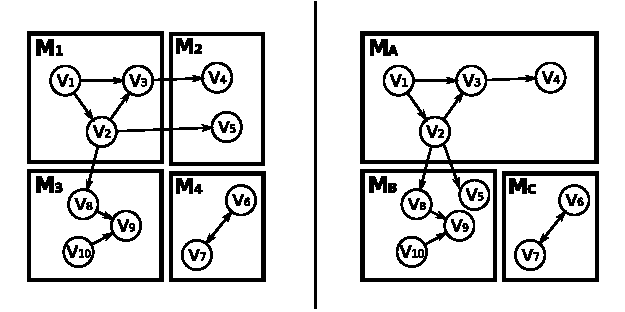
\includegraphics[scale=1]{figuras/redes-dupla}
	\caption{Dois agrupamentos de um mesmo sistema de software hipotético, descrito como um grafo que representa dependências entre classes.}
	\label{fig:mojo}
\end{figure}

% É fácil verificar se dois agrupamentos de um mesmo conjunto de entidades são idênticos ou não. Para comparar diferentes agrupamentos produzidos por algoritmos, no entanto, é preciso definir uma métrica de similaridade entre agrupamentos que seja capaz de determinar qual agrupamento de uma coleção de agrupamentos é mais similar a um agrupamento de referência.

A ideia por trás da métrica MoJo é que um agrupamento dado é muito similar a um agrupamento de referência se é possível transformar o primeiro agrupamento no segundo usando poucas operações do tipo mover e mesclar. A operação mover consiste de mover uma entidade de um módulo para outro módulo distinto. A operação mesclar consiste de mesclar dois módulos. O MoJo entre  dois agrupamentos é igual ao número de operações de mover e mesclar que são necessárias para transformar o primeiro agrupamento no segundo. Quanto menor o MoJo, maior a similaridade entre dois agrupamentos; agrupamentos idênticos têm MoJo igual a zero.

% A métrica MoJo não é simétrica. Para chegar a essa conclusão, basta observar que há uma operação de mesclar módulos, mas não uma operação de dividir um módulo em dois. No contexto de avaliação de algoritmos de agrupamento de software, é considerado o número de operações necessárias para transformar o agrupamento encontrado por um algoritmo no agrupamento de referência, e não o contrário.

Na Figura \ref{fig:mojo}, considerando que o agrupamento de referência é o segundo (o da direita), o MoJo entre os dois agrupamentos vale 2. Para transformar o primeiro agrupamento no segundo são necessárias, portanto, duas operações: mesclar os módulos $M_1$ e $M_2$, e mover o vértice $v_5$ para o módulo $M_3$. Após a realização dessas operações, os agrupamentos se tornam idênticos, considerando as correspondências $(M_1 \cup M_2) = M_A$, $M_3 = M_B$ e $M_4 = M_C$.

Observando que o valor MoJo entre dois agrupamentos com o mesmo número de entidades varia entre 0 e o número de entidades em cada agrupamento, $n$, é possível definir uma métrica, chamada MoJoSim, que mapeia o valor MoJo em uma escala de 0 a 1 \cite{Bittencourt2009}. O valor 0 representa a menor similaridade e o valor 1, a maior similaridade. O valor de MoJoSim entre dois agrupamentos é definido de acordo com a seguinte equação:

$$
\mathrm{MoJoSim}(X, Y) ~=~ 1 - \frac{\mathrm{MoJo}(X, Y)}{n}
$$

O valor de MoJoSim na Figura \ref{fig:mojo} é, portanto, igual a $1 - \frac{2}{10} = 0,8$.

% Anquetil avaliou 

% Movido
% Wu, Hassan e Holt \cite{Wu2005} avaliaram os algoritmos Bunch, ACDC e algoritmos aglomerativos comparando, através da métrica MoJo, os agrupamentos encontrados pelos algoritmos com agrupamentos de referência de 5 sistemas de software em C e C++, representados como um grafo dos arquivos fonte e dependências estáticas entre os arquivos. Os agrupamentos de referência foram obtidos automaticamente a partir de uma análise da estrutura de diretórios dos sistemas. Cada diretório contendo pelo menos 5 arquivos fonte foi considerado um módulo do sistema. Bittencourt e Guerrero \cite{Bittencourt2009} realizaram um experimento semelhante, porém avaliando algoritmos de agrupamento estudados em outros domínios aplicados sobre um conjunto de 4 sistemas em Java.

\end{chapter}

%%%%%%%%%%%%%%%%%%%%%%%%%%%%%%%%%%%%%%%%%%%%%%%%%%%%%%%%%%%%%%%%%%%%%%%%%%%%%%%%

\end{document}